\documentclass[]{article}
\usepackage{natbib}
\usepackage{amsmath}
\usepackage{amssymb}
\usepackage{amsthm}
\usepackage{setspace}
\usepackage{palatino}
\usepackage{graphicx}
\usepackage[font=small,labelfont=bf]{caption}
\usepackage{titlesec}

%Theorems
\theoremstyle{plain}
\newtheorem{thm}{Theorem}[section]
\newtheorem{lem}[thm]{Lemma}
\newtheorem{prop}{Proposition}
\newtheorem*{cor}{Corollary}
\newtheorem{assumption}{Assumption}


\title{The Geographic Bias of Growth and Structural Change}
\author{James Macek}
\onehalfspacing
\bibliographystyle{chicago}


\usepackage{hyperref} %Load hyperref last for footnote linking to work as intended. 
%Colours for hyperreferencing
\hypersetup{
colorlinks=true,
linkcolor=blue,
filecolor=blue,      
urlcolor=blue,
citecolor=blue,
}

\begin{document}
\maketitle

\begin{abstract}


\end{abstract}

\newpage
%%%%%%%%%%%%%%%%%%%%%%%%%%%___INTRODUCTION____%%%%%%%%%%%%%%%%%%%%%%%%%%%%%%%%%%%%%%%%
\section{Introduction}

\paragraph*{}
Contemporary models of spatial equilibrium imply that productivity growth, when uniform across locations, does not change the overall distribution of economic activity in space. In this paper, I argue that this feature masks an important mechanism by which growth concentrates economic activity even when the spatial distribution of productivity remains unchanged. 
\paragraph*{}
The theory rests on two ideas. Firstly, growth changes the consumption basket; shifting expenditures away from food and toward other goods. This manifests in general equilibrium as \textit{structural change}, where agricultural employment falls relative to other sectors as the economy grows. On the other hand, demand for agriculture shapes geography insofar as the returns to concentrating it in space are dwarfed by other sectors. Taken together, these imply that workers leaving agriculture during the structural change process are absorbed by regions with high population density. This reallocation increases the dispersion of population density across space.
\paragraph*{}
This link between structural transformation and urbanization has previously been explored in \citet{urbstruct}. They build a theory and rationalize rising spatial concentration in part by appealing to differences in land intensity across sectors. As a result, population dense regions specialize outside of agriculture under trade and, conditional on specializing, tend to have more dispersion in population densities. I build on this research in two ways. As a small contribution, I  provide conditions on the strength of agglomeration and productivity growth and explicitly prove this relationship holds. Secondly, and most importantly, I measure the magnitude of this effect by taking a spatial equilibrium model to Chinese data from 2000-2005. The theory reveals how to make this measurement. 
\paragraph*{}
The structural model allows for falling migration, regional trade costs and changing relative productivity as alternative explanations for the reallocation of workers across space. I find that productivity growth, when uniform across locations and set to the inferred average level, accounts for approximately 38 percent of the total rise in population density dispersion predicted by the model\footnote{The model I use is nonlinear, so there is some ambiguity surrounding the allocation of marginal effects between productivity growth, trade and migration costs. I report the Shapely decomposition here.}. In addition, the model is not calibrated to match the observed rise in population density dispersion, but accounts for over half of it.
 \paragraph*{}
 Why study China? During this period, the country saw a massive reallocation of workers toward the population-dense coastal provinces, such as Beijing, Shanghai and Guangdong. Such mobility was and is made exceptionally difficult by a unique institution-- the Hukou system \citep{Chinashukou60} \citep{hukoulaboutcome}. However, by the 2000's the Chinese government introduced significant reform, and there is some quantitative evidence that these reforms caused migration inflows \citep{Fan2018HukouRI}. At the very least, migration costs (measured by observing spatial differences in real income relative to migration flows) fell significantly during the period \citep{tombezhu}. These falling migration costs can increase the dispersion of population density as more workers arbitrage away spatial differences in real income. Moreover, \citet{tombezhu} also find that falling trade costs during this period were also significant; and falling trade costs are key in determining the spatial distribution of economic activity in the economic geography literature. How does the impact of the theory stack up against these two variables, which themselves are largely influenced by policy? China provides a unique opportunity to answer this question.
 \paragraph*{}
 At the same time, China also experienced rapid growth and structural change during this period.  These facts alone distinguish it as a country where the geographic bias of growth could play a major role in shaping the population distribution.
\paragraph*{}
The strategy behind calibrating this model starts with the fact that \textit{relative} productivity growth across space is identified using regional trade data and a gravity model. However, this procedure is uninformative about \textit{aggregate} growth-- that is, a scale factor that determines productivity in absolute terms. I propose an estimation strategy that disciplines this growth using information contained in falling agricultural spending. First, I estimate income and substitution elasticities over agricultural goods using GDP data and prices inferred from the gravity model. Given these estimates, I choose the level of aggregate productivity growth that matches the fall in average agricultural spending observed in the data. 
\paragraph*{}
For other parameters, calibration uses recent methodology in the trade and spatial literature. Trade costs are mapped from provincial trade data and standard estimates of the trade elasticity. Combined with the calibrated productivity, these are used to construct measures of real income per capita implied by the model. Migration frictions are then inferred from the discrepancy between differences in real income and the observed movement of workers from their hukou.

\paragraph*{}
The paper is organized as follows. I review the literature in Section \ref{section:literature}, provide a description of the data and some key motivating facts in Section \ref{section:datafacts}, present a theory and prove it can explain these facts in Section \ref{section:theory}, and employ the structural model in Sections \ref{section:structmodel}, \ref{sect:calibration} and \ref{section:results}. Section \ref{section:conclusion} concludes.

%%%%%%%%%%%%%%%%%%%%%%%%%%%%%%%LITERATURE%%%%%%%%%%%%%%%%%%%%%%%%%%%%%%%%%%%%%%
\section{Literature}\label{section:literature}
\paragraph*{}
This paper lies at the heart of a budding literature on the interplay between structural change and geographic outcomes. The earliest of these frames structural change as the driver for spatial convergence in US earnings before 2000 \citep{casellicoleman}, which has subsequently been applied in China after 2000 \citep{hao2020}. In contrast to these papers, I focus on the population distribution rather than falling inequality. As a result, they do not emphasize the weaker returns to concentrating agriculture in space as I do. 
\paragraph*{}
Another strand of literature throws international trade integration into the mix. \citet{urbwoindustrialization} show that specialization in non-industrial sectors under trade lead to higher non-traded goods employment in "consumption cities"; though space is not directly modeled. \citet{rfargentina} show that regions more integrated into world markets exhibit low agricultural employment shares because of both differences in land intensity and rising employment in non-traded sectors. Data limitations do not allow me to consider the Balassa-Samuelson effect central to these papers. In addition, while I don't focus on international trade in the theory, it is empirically a force for suppressing agricultural employment in the coastal provinces because they import a significant amount of food\footnote{In the context of China, local specialization under trade is in part determined by proximity to the eastern coast, highlighed in \cite{cosarfagjelbaum}.}.
\paragraph*{}
This literature also highlights dynamic productivity diffusion in space as drivers of structural change \citep{spatdev}  \citep{delventhalglobenet}. I abstract from the main mechanisms in these papers by using a simple model of local increasing returns. 
\paragraph*{}
Of this body of work, the most closely related are \citet{urbstruct}, \citet{MURATA2008} and \citet{eckertpeters}, whom explicitly study the effect of structural change on geography. I build on the mechanism driving spatial concentration in the first two by linking theory to a structural model and assessing it quantitatively against competing hypotheses. The third contains a negative result; that the spatial reallocation of workers accounted for essentially zero of US structural transformation since 1880. In contrast, I ask how falling agricultural employment accounts for total spatial reallocation toward dense locales. I also emphasize the link between density and specialization outside of agriculture, which they do not. In the following section, I show that the empirical observation in \cite{eckertpeters} holds in China, and that it is consistent with structural change accounting for sizable portion of rising concentration in the period that I study. 
\paragraph*{}
This paper is nested within the broader literature on structural change, growth and the agricultural productivity gap\footnote{See \citet{hrvch6} for a recent review of the structural change literature. This includes \citet{ngaipissa}, \citet{boppart2014}, \citet{cominetal2021}, \citet{matsuyama1992, matsuyama2009, engelslawglobal}, \citet{uy2013}, \citet{bustos1996etal}, \citet{bustos2020etal}, \citet{swiecki2017}, \citet{loganetal}, \citet{cravinosotelo}  and \citet{duarterestuccia}.}. The general concern of these papers are macroeconomic outcomes, and use models where there are multiple sectors but no notion of space within countries\footnote{A notable exception is \citet{karadi2017cattle}, which links a disaggregated equilibrium in a monocentric city model to the aggregate production function to facilitate development accounting. While the research question is fundamentally different, their model also features a version of the spatial bias of growth -- see Proposition 3.}. However, the models that give rise to structural change are central to the equilibrium geography that I study here. In particular, I use the non-homothetic CES preferences of \citet{cominetal2021} and \citet{loganetal} and adapt their estimation strategy for to use with prices inferred from trade data. 
\paragraph*{}
While the model and methodology in this paper may come from elsewhere, I study a central question in economic geography -- how is the distribution of economic activity in space determined? I build on the models of \citet{krugman1991}, \citet{PUGA1999}, \citet{aggtraderev}, \citet{MURATA2008}, \citet{donalddavishme} and subsequent work to answer this question. I also draw from recent spatial models that are rich enough to have an empirical implementation, including \citet{allenarkolakis}, \citet{redding2016}, \citet{nagyhinterlands}, \citet{pathdep}, \citet{geodev}, \citet{sotello2020}, \cite{eckertpeters} and importantly \citet{tombezhu}, \citet{hao2020}, \citet{MA2020} and \cite{Fan2019} in the context of China. Each employ a scheme to map observed data to unobservable parameters, which I use extensively for productivity, trade and migration costs. In particular, I draw heavily from the methodology and data choices in \citet{tombezhu}. The point of departure is the use of homothetic preferences\footnote{With the exception of \cite{hao2020}.}, so that any spatially uniform scaling of productivity do not change the equilibrium outcomes that I study. I generalize these empirical implementations to a model falling outside this common class.  
\paragraph*{}
Surrounding this central question is an empirically oriented literature in which transportation infrastructure is the main dependent variable. These include \citet{baumsnow2007}, \citet{durturner}, \citet{durturnerurb}, \citet{bs2020}, \citet{herzog2021}, \citet{faberb}, \citet{bart2018} and in particular \cite{bsetal2017} and \cite{bsetal2020} in the Chinese context. I compare the magnitude of the spatial bias of growth against the effects of falling trade costs (among other benefits) considered in these papers. Moreover, data constraints force me to consider a large level of spatial aggregation than what is typical. I hope to consider a model with prefectures instead of provinces in future work.   

\section{Data and Facts}\label{section:datafacts}
\paragraph*{}
 The data reveal key features of China's growth that link geographic concentration and structural change. Firstly, I document rising spatial concentration that is \textit{purely} driven by employment growth outside of agriculture. I also show that locations with higher population density tend to have lower agricultural employment shares and a revealed comparative advantage outside of agriculture in the cross section. These relationships have a clear grounding in the theory I present in the following section.
\paragraph*{}
To construct these facts, I draw on multiple data sources at the provincial level, excluding Tibet. These concern provincial and international trade, migration, capital, agricultural spending and GDP data disaggregated by the primary and non-primary industries. In the Chinese census and China Statistical Yearbooks (CSY), the primary industry is an aggregate of farming, animal husbandry, forestry and fishing. I follow \cite{hao2020} by defining the primary industry as the agricultural sector, and all other economic activity as an aggregated non-agricultural sector.
\paragraph*{}
I exploit a model of trade to calibrate productivity, which requires provincial and international trade data. These flows come from the 2002 and 2007 regional input-output tables, which are disaggregated by sector. These are the same data used in \cite{Fan2019} and \cite{tombezhu}. However, this level of disaggregation comes at a disadvantage. Flows are limited to rail transport, which misses a bulk of trade. 
\paragraph*{}
To capture imperfect labour mobility, I use migration data from the 2000 and 2005 Chinese population censuses. These data map individuals residing in a province and sector to their hukou. I measure migration flows as the fraction working in a sector or province different from the hukou, in the same way as \cite{tombezhu} and \cite{hao2020}. Without loss of generality, I use the term "agricultural" in reference to the rural hukou. Interpreting the movement of workers across sectors but not space as migration is not necessary; the model has no notion of space \textit{within} provinces.
\paragraph*{}
Value added and labour employment data come from the CSY. I use the capital data from \cite{hao2020}, whom construct it using observed investment. I do not observe good measures of land use, so I infer it as the allocation that equalizes the return to land within provinces. I also assume that the entire official landmass is used for either production or consumption, which is also reported in the CSY. 
\paragraph*{}
Food spending shares are split by urban and rural areas within each province using data from \textit{China Data Online}. I ascribe rural spending shares to agricultural workers and urban to workers outside agriculture, similarly to \cite{hao2020}. This is not a perfect match, because workers in rural areas within a province may be employed outside of agriculture. However, it is a sensible one -- an overwhelming majority of those holding rural hukou are employed in the primary sector. These food spending shares appear quite large (on average 30 percent in 2000) because I use after tax income. This potentially ignores income effects stemming from the provision of goods and services by the government sector.  

\subsection*{The primary sector and rising spatial concentration}
\paragraph*{}
How much has spatial concentration risen from 2000 to 2005? When measuring it as the coefficient of variation of employment density across provinces, it increased from 1.1 to 1.218, representing an approximate 10 percent rise in just 5 years\footnote{When measuring this as employment weighted population density dispersion, it increased from 0.714 to 0.806.}. To put in perspective, I compare this to the US. At the Minor Civil Division level of aggregation, the same statistic increased from 0.3716 to 0.506 from 1880-2000 -- representing a growth of 36 percent in a period of \textit{120 years} \citep{urbstruct}. Extrapolating the observation in China to this longer time period implies a growth of almost 1000 percent\footnote{This extrapolation is simply for comparison. The rise in population density dispersion was transitory -- it vanished completely from 2005-2010. Explaining this observation is outside the scope of the paper.}. 

\paragraph*{}
The rising spatial concentration can be illustrated with a regression of employment growth on initial employment density. If employment growth is on average larger for more population dense locations, then population density dispersion will tend to rise. A plot of the regression and the data is reported in Figure \ref{fig:emp_dens_growth}. The positive coefficient is clearly driven by the inclusion of exceptionally fast growing provinces, like Shanghai, Beijing and Guangdong. 

\begin{center}
\begin{figure}[h]
	\centering
	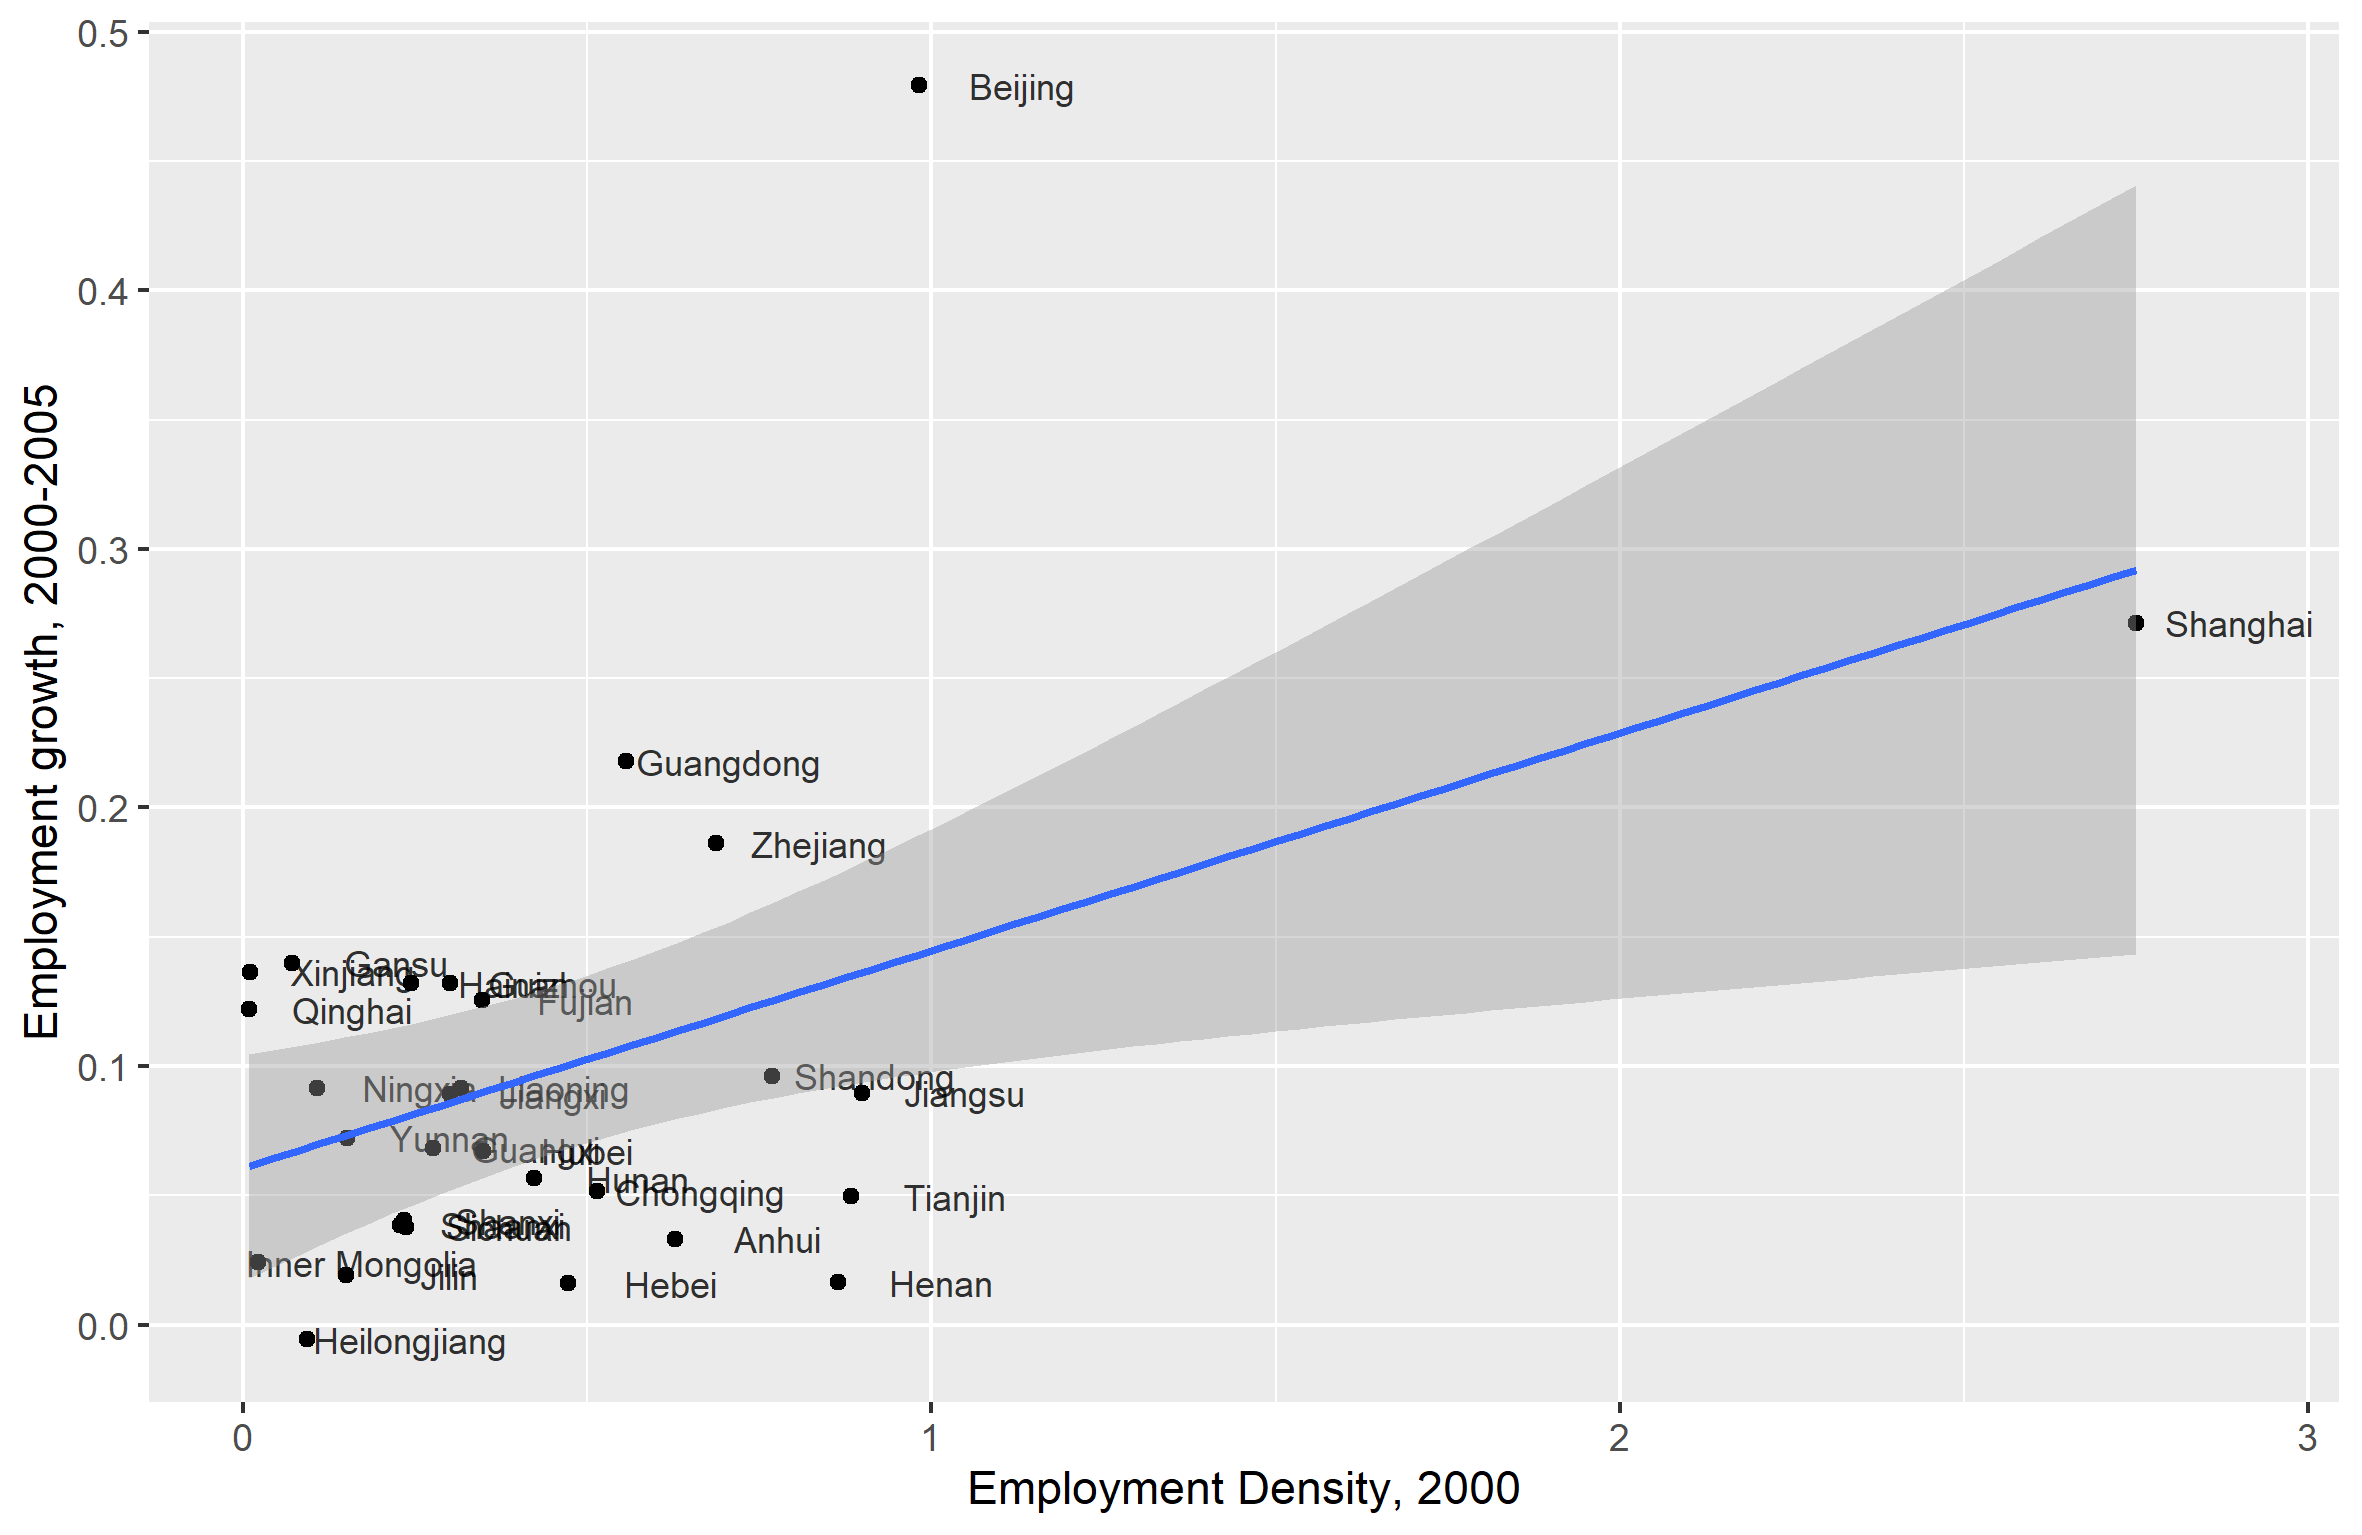
\includegraphics[width=0.8\textwidth]{emp_growth_density.png}
	\caption{Relationship between average employment growth and employment density by Chinese province. Density is measured in millions per 1000 square miles. Slope estimate for unweighted and employment-weighted is 0.0841 and 0.0633, respectively.  Unweighted and employment weighted regressions have a p value of $<$ 0.01 and 0.08.}
	\label{fig:emp_dens_growth}
\end{figure}
\end{center}

\paragraph*{}
Which sectors are driving the rising concentration? To explore this, I decompose the total employment growth rate $g_{i}$ into a \textit{agriculture} (a) and \textit{non-agriculture} (n) components. These are related in the following way,

\begin{equation*}
g_{i} = g_{i, a}s_{ia, 2000} + g_{i, n}s_{in, 2000}
\end{equation*}
where $g_{i, s}$ and $s_{is, 2000}$ are the growth rates of employment and the share of employment in 2000 in sector $s$ and province $i$, respectively. I regress both of these components against initial employment density separately, noting that the coefficients on each regression must add up to the slope reported in Figure \ref{fig:emp_dens_growth}. I find that the slope for the agricultural component is negative, implying that the relationship is entirely driven by activity outside of the primary sector. A plot of both regressions is reported in Figure \ref{fig:na_emp_dens_growth}.

\begin{center}
	\begin{figure}[h]
		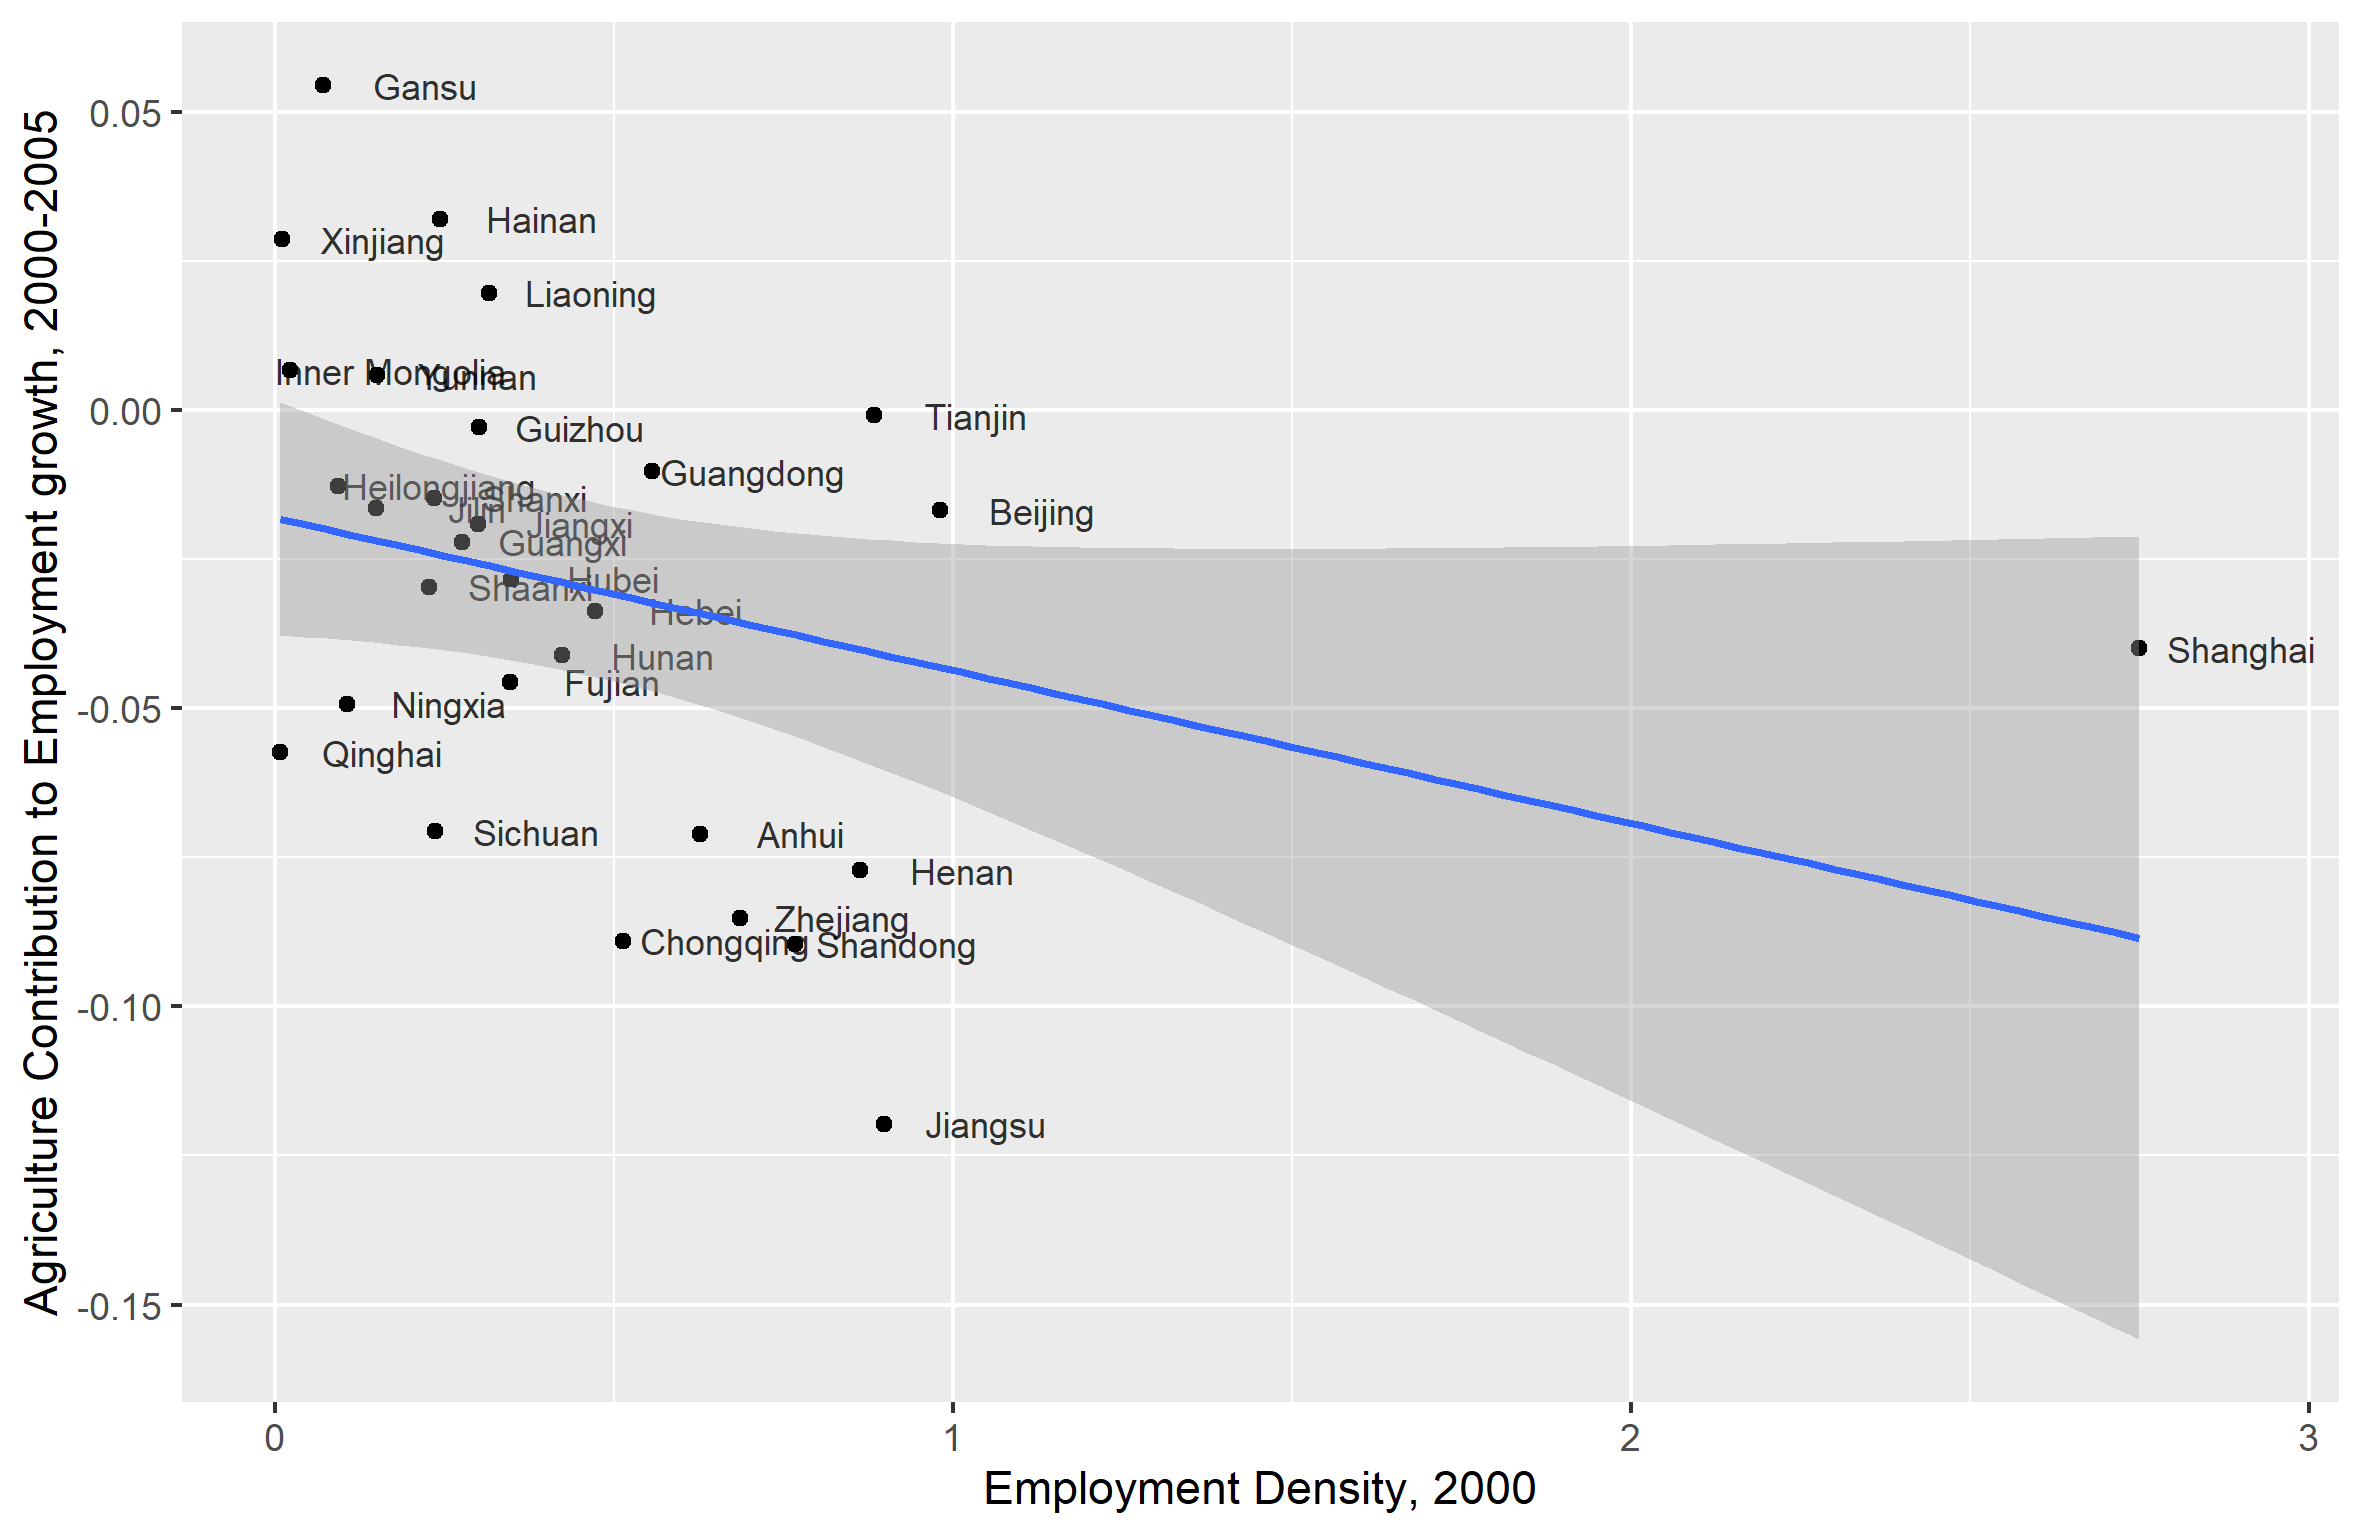
\includegraphics[width=0.5\textwidth]{ag_cont_growth_density.png}
		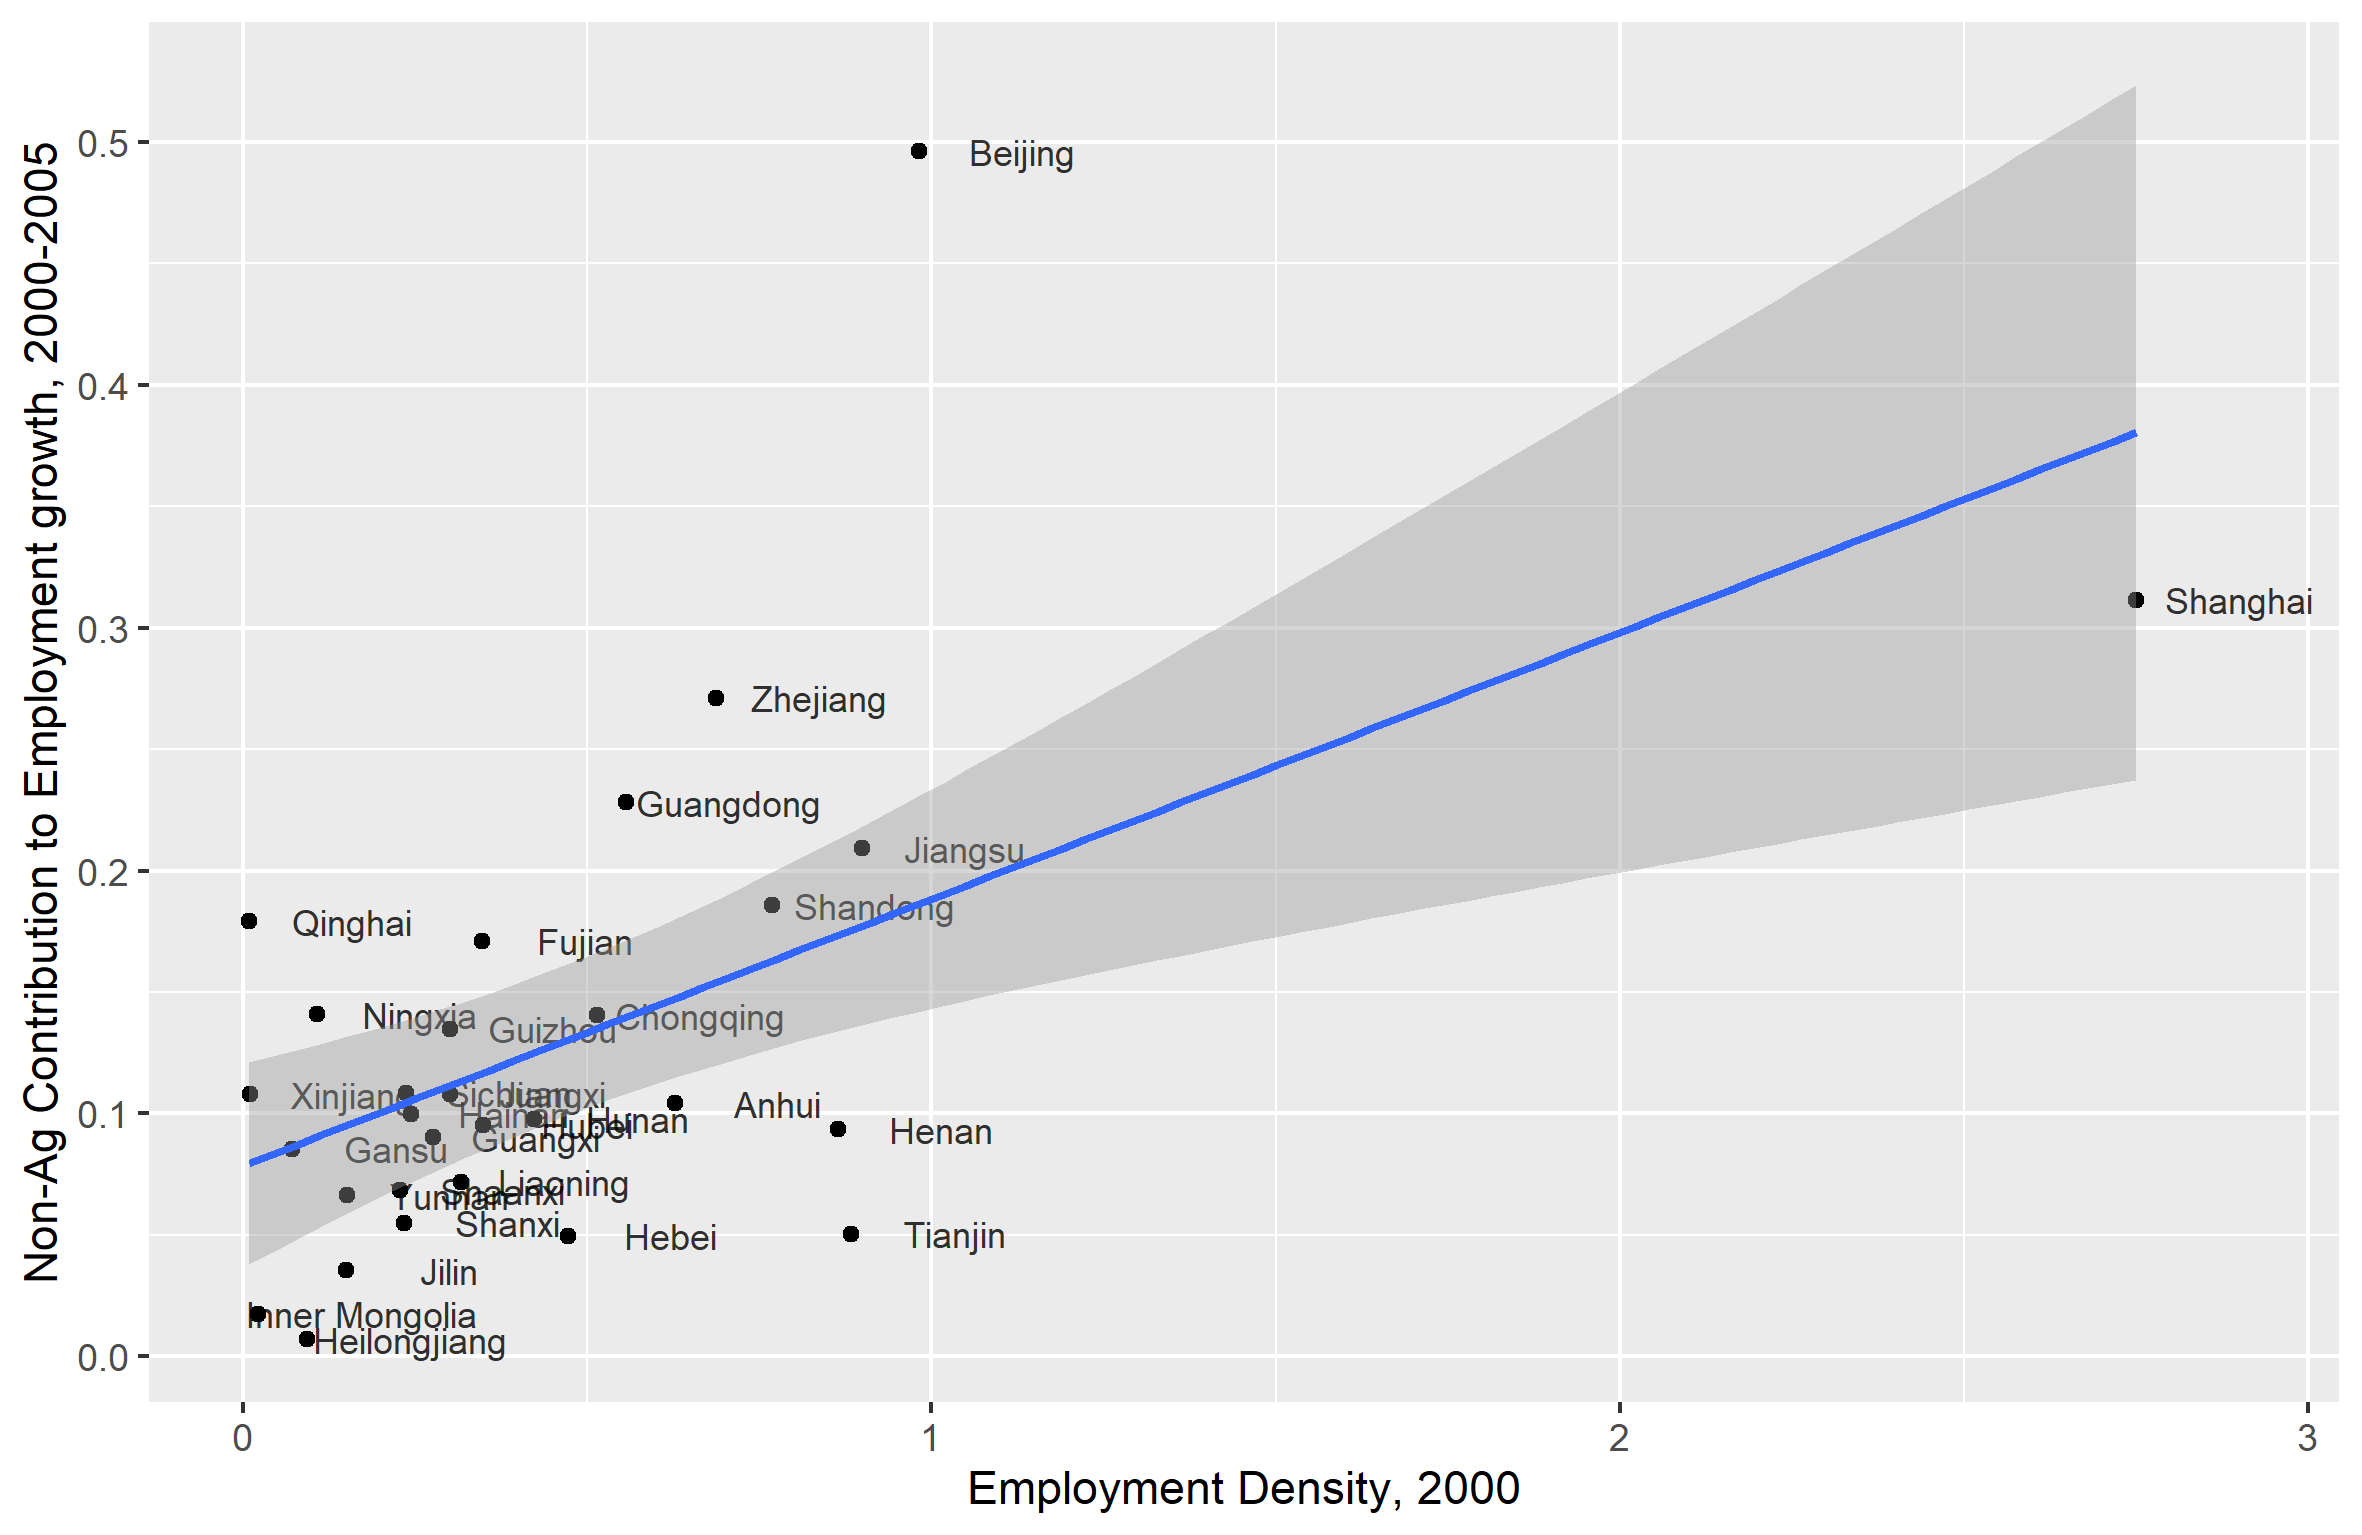
\includegraphics[width=0.5\textwidth]{na_cont_growth_density.png}
		\caption{Relationship between employment growth by sector and employment density by Chinese province. Density is measured in millions per 1000 square miles. Employment-weighted slope estimates are -0.0593 and 0.1226 for the agricultural and non-agricultural components, with similar magnitudes for the unweighted regressions. Non-ag weighted and unweighted regressions have a p-value of $<$ 0.01 and 0.02, respectively.}
		\label{fig:na_emp_dens_growth}
	\end{figure}
\end{center}

\paragraph*{}
The facts shown in Figures \ref{fig:emp_dens_growth} and \ref{fig:na_emp_dens_growth} are readily explained by the interplay between structural change and the differential returns in space across sectors. Structural change causes outflows of labour from the agriculture, and these outflows tend to have a relationship with population density that is relatively weaker in magnitude\footnote{The agriculture slope estimate in Figure \ref{fig:na_emp_dens_growth} has less than half the magnitude than that of the non-agriculture component.}. These workers tend to get absorbed in provinces with a comparative advantage outside of agriculture. But, comparative advantage is in part determined by density insofar as the local supply of land in production is inelastic. The question remains -- is the relationship between density and comparative advantage a feature of the data? I document below. 
\paragraph*{}
Before continuing, I note an additional caveat. These results may appear at odds with the motivating evidence in \cite{eckertpeters}, but I show that they are not. I repeat their additive decomposition of aggregate structural change into "spatial reallocation" and "regional transformation" components, defined by
\begin{equation}
	s_{a, 2005} - s_{a, 2000} = \sum_{i}\big[s_{ia, 2000}(l_{i, 2005} - l_{i, 2000}) + (s_{ia, 2005} - s_{ia, 2000})l_{i, 2005}\bigg]
\end{equation}
where $s_{at}$ is the aggregate employment share in agriculture at time $t$, and $l_{it}$ the fraction of employment in province $i$ at time $t$, respectively. Intuitively, if the spatial reallocation term $\sum_{i}s_{ia, 2000}(l_{i, 2005} - l_{i, 2000})$ is relatively large, then most of the structural transformation comprises of workers moving across provinces. I find that the term  accounts for only 5 percent of the total change in the share of agricultural employment. This is approximately the same number they find in the US between 1880 and 2000. I reiterate that, while spatial reallocation may not account for much of China's structural transformation, structural transformation may significantly affect spatial reallocation toward dense provinces. This is precisely what Figure \ref{fig:na_emp_dens_growth} suggests.

%\paragraph*{}
%In addition, employment growth may be driven not by population growth but by labour supply decisions. This is an issue because there is no clear way to assign the unemployed or non-participants to sectors, which are required for the decomposition in Figure \ref{fig:na_emp_dens_growth}. If the relationship were driven by the intensive margin of labour supply, that would be interesting in its own right. However, the mass migration documented in this period does not corroborate this alternative explanation, see \cite{tombezhu}, \cite{hao2020} and \cite{Fan2019}.    
 
\subsection*{Structural change, specialization and comparative advantage}
\paragraph*{}
How fast was structural change during this period? The aggregate employment share in agriculture fell from 52.9 percent to 44.8 percent. This decrease is in part reflected in the falling aggregate food expenditure shares implied by the provincial data. Food represented 31.8 percent of the aggregate budget in 2000, and decreased to 28.2 percent in 2005. 
\paragraph*{}
How has structural change varied by density, and does this reflect comparative advantage? To examine the relationship in the cross section, I plot the 2000 agricultural employment share against employment density in Figure \ref{fig:emp_share_dens} of Appendix \ref{appendix:figures}. The relationship is strong. Each additional million people per thousand square miles is associated with a 0.19 decrease in the share of agriculture employment in the range of densities observed in the data. This relationship remains stable in transition to 2005.   
\paragraph*{}
The relation in Figure \ref{fig:emp_share_dens} can be rationalized in the absence of trade. Spatial differences in equilibrium real income could induce this pattern whenever migration is costly. Instead, I consider a more direct measure -- the Revealed Comparative Advantage (RCA) as in \cite{balassa}. As is well known, it is defined as follows for province $i$ and sector $s$, 
\begin{equation*}
	RCA_{i, s} = \frac{E_{i, s}/\sum_{s' \in \{a, n\}}E_{i, s'}}{\sum_{i' \in \mathbf{P}}E_{i', s}/\sum_{s' \in \{a, n\}, i' \in \mathbf{P}}E_{i', s'}}
\end{equation*} 
where $E_{i, s}$ are exports and $\mathbf{P}$ is the set of province indices and a rest-of-the-world aggregate. Exports in this case are defined to include regional trade. In words, RCA measures how intensively a province exports goods in $s$ relative to how intensively that good is exported worldwide. I plot a regression of RCA in agriculture on employment density in 2000, see Figure \ref{fig:RCA}. It reveals that density accounts for about 30 percent of the variation in revealed comparative advantage in the data. In addition, this correlation is supplemented by evidence in \cite{bsetal2020}. They show that improved road infrastructure (which presumably increases regional trade integration) caused smaller prefectures to specialize in agriculture.
\paragraph*{}
In short, density matters for trade patterns. Like the previous fact, this is grounded in theory. Chinese agriculture uses land more intensively with a cost share of 0.26 relative to 0.01 in non-agriculture \citep{hao2020}. If the supply of land for use in agriculture is inelastic and agglomeration forces do not vary too widely by sector, this means that high land prices in dense locations will crowd out agricultural activity.
\begin{center}
	\begin{figure}[h]
		\centering
		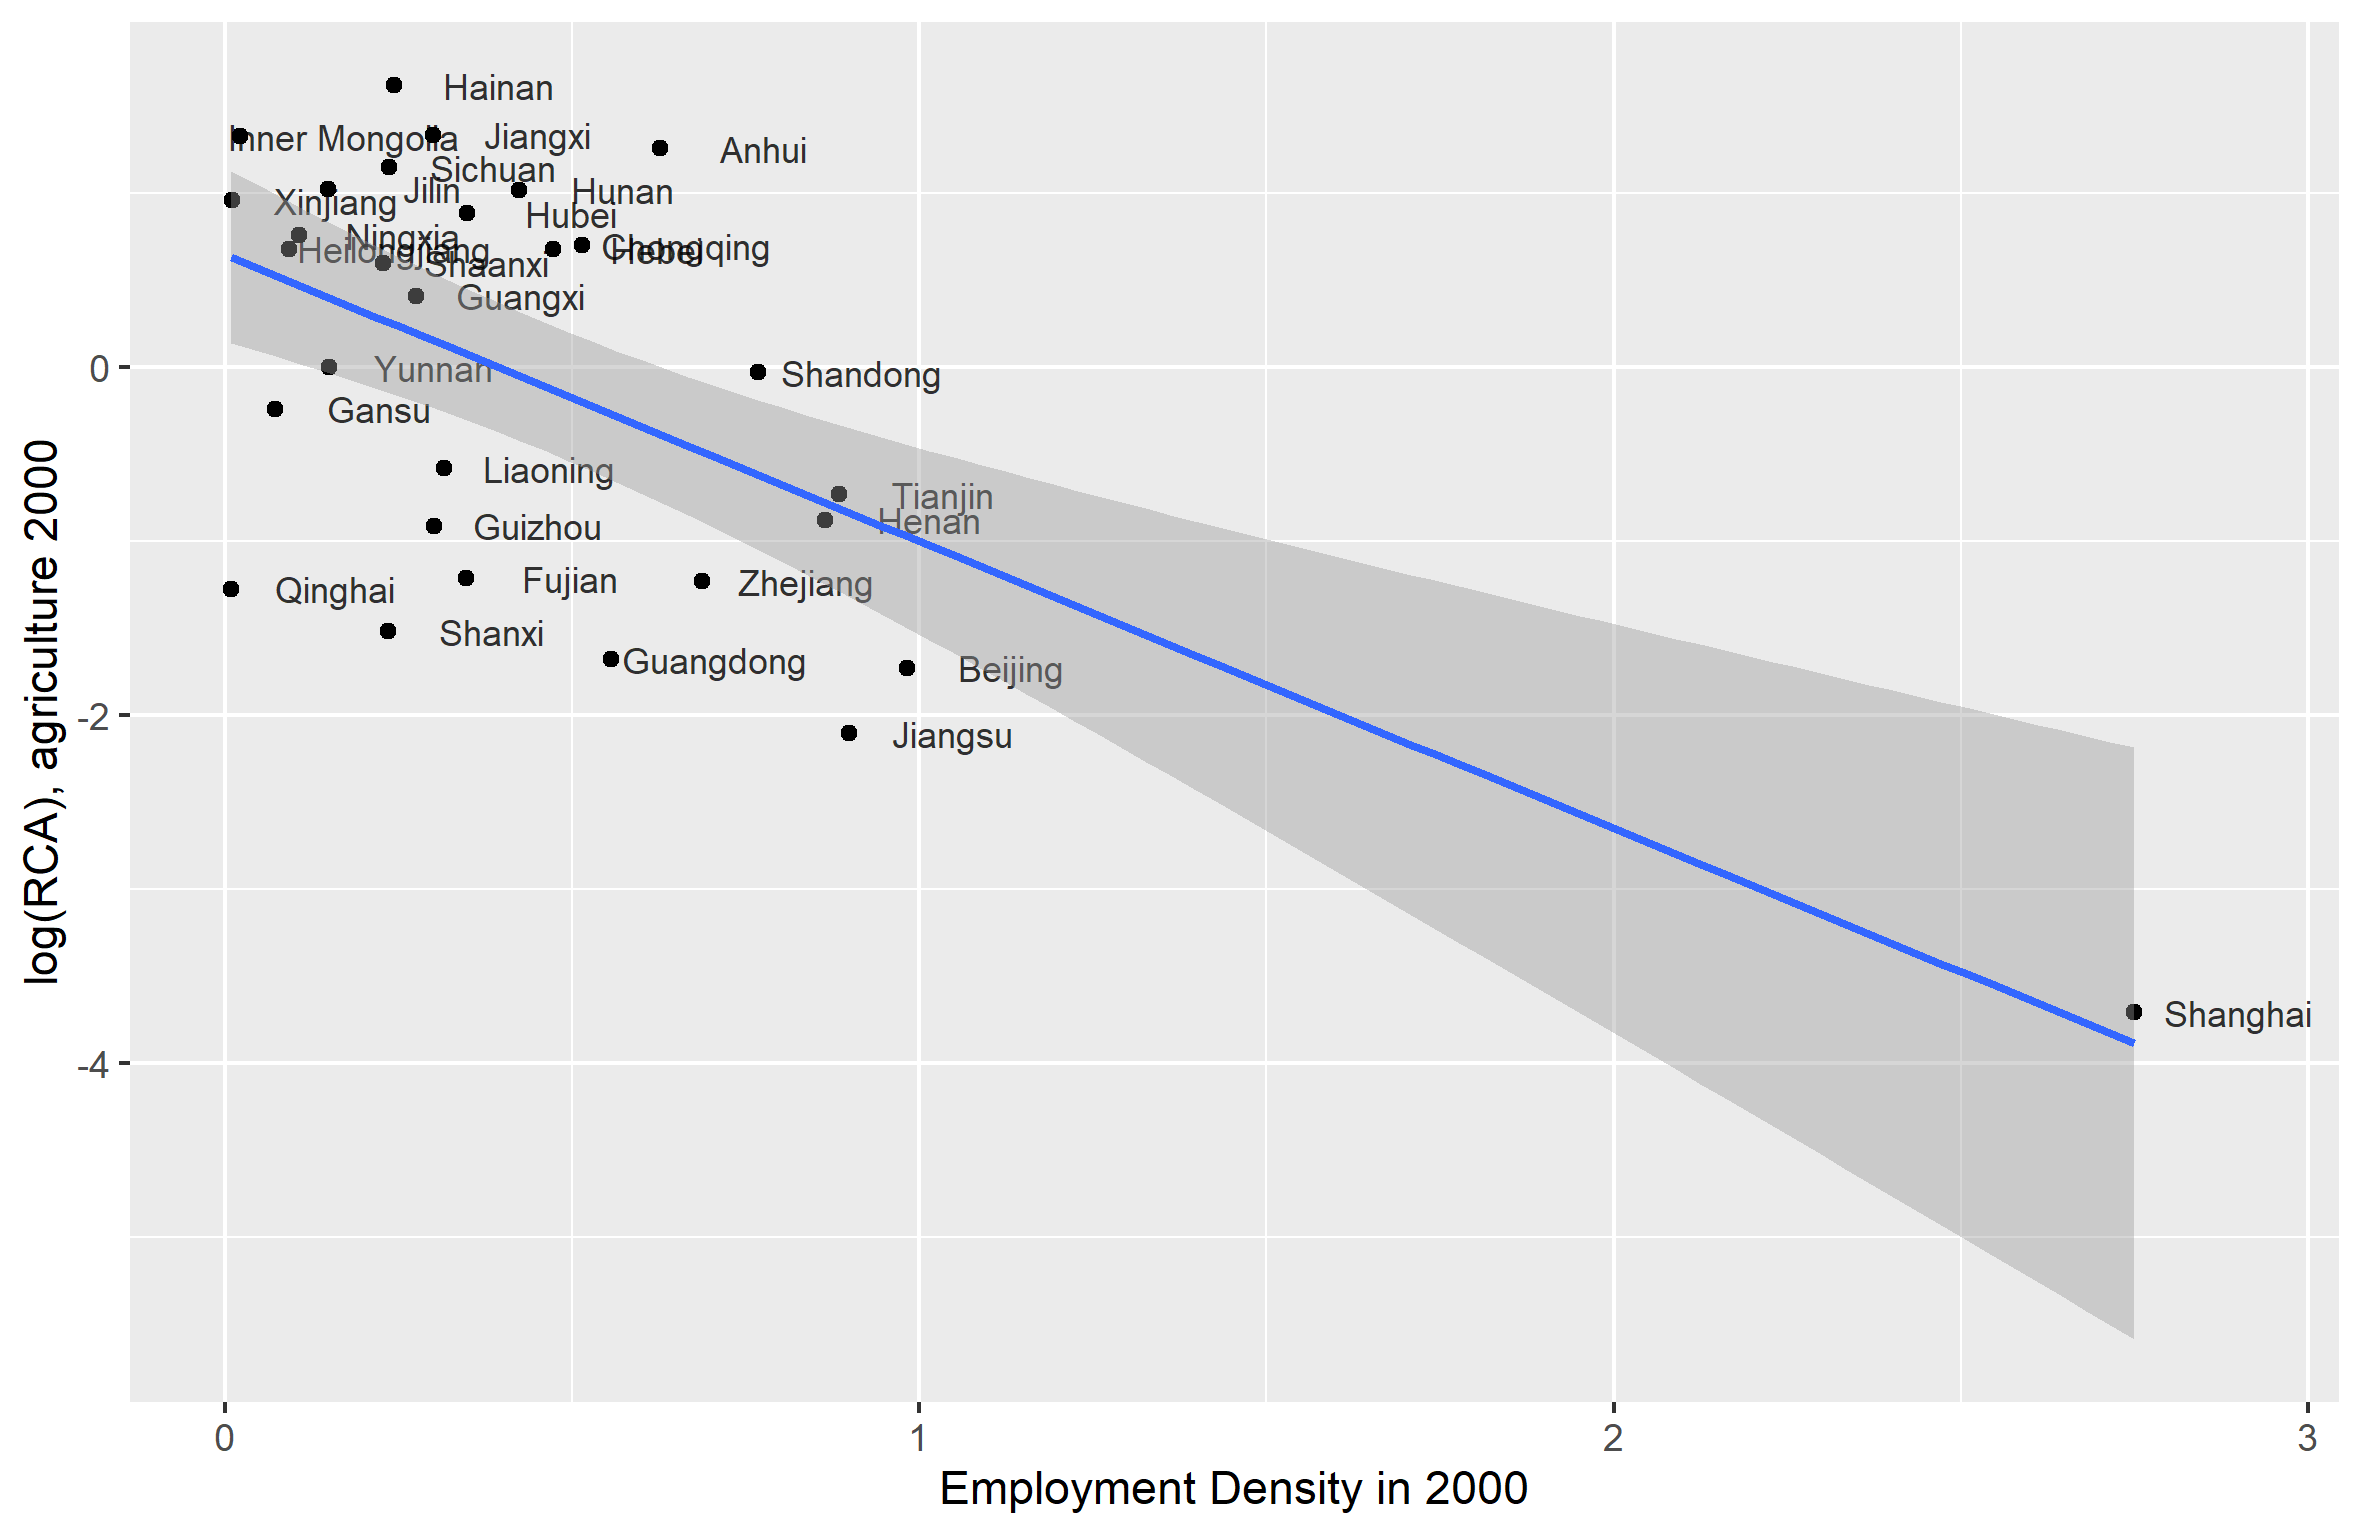
\includegraphics[width=0.8\textwidth]{figRCA.png}
		\caption{Relationship between revealed comparative advantage and employment density by Chinese province. Density is measured in millions per 1000 square miles. The slope estimate is -1.899 with a p-value of $<$ 0.0001, and the regression has an $R^{2}$ of 0.3. Similar results hold in the 2005 cross-section. }
		\label{fig:RCA}
	\end{figure}
\end{center}
%\subsection*{Alternative explanations}
%Coming soon. A run down of how trade costs, migration costs and other explanations can give rise to the results we see %here. Motivates use of structural model.

%%%%%%%%%%%%%%%THEORY%%%%%%%%%%%%%%%%%%%%%%%%%%%%%%%%%%%%%%
\section{Theory}\label{section:theory}
\paragraph*{}
Explaining these facts and guiding the methodology behind the empirical work, I introduce a theory that captures when and how the geographic bias of growth will occur, and how to measure it. At the heart of this theory is the idea that concentrating agriculture in space comes with a penalty that is larger than other sectors. As a result, the intensity of agricultural consumption (or equivalently, employment in general equilibrium) will inversely affect how concentrated the geography will be. Structural change thus increases concentration. 
\paragraph*{}
 The theory assumes exogenous spatial variation in productivity. I make this assumption in part because productivity differences are evident, and persist in the time period I study.  Moreover, the inferred differences across provinces cannot be explained by population density using typical estimates of the agglomeration elasticity\footnote{See \citet{combesg2015} for a review of the literature on the estimation of agglomeration elasticities.}. I use productivity differences solely to generate spatial variation in economic activity. 

\paragraph*{}
To this end, define the set of locations $\{1, 2\}$ indexed by $i$, a set of sectors $\{a, n\}$ indexed by $s$, and assume there are a measure $L$ workers to be allocated to each of these sector-location pairs. Each location is endowed with $H$ units of land that can be allocated to each sector, but are immobile across space\footnote{Equivalently, the model could be solved with arbitrary land endowments. Then, I can normalize land in each location to 1 and express the labour allocation relative to its total land endowment.}. 

\subsection*{Production}
\paragraph*{}
 Each sector-location uses a Cobb-Douglas technology
\begin{equation*}
	Y_{i, s} := A_{i, s}L_{i, s}^{1-\beta_{s}}H_{i, s}^{\beta_{s}}
\end{equation*}
where $A_{i,s} := a_{i, s}\big(\frac{L_{i, s}}{H_{i, s}}\big)^{\alpha_{s}}$ captures economies of density that are not internalized by the representative firm. I assume land is used more intensively in agriculture, $1 >\beta_{a} > \beta_{n} > 0$, and positive economies of density $\alpha_{s} > 0$.  To abstract from Ricardian motives for specialization, I assume that location $1$ and $2$ have productivity $ca_{s}$ and $a_{s}$ in each sector $s$ and $c>1$, respectively. In other words, there are no differences in relative productivity across sectors. However, differences in relative marginal costs will arise. This is because location $1$ must have more workers in an equilibrium where mobility is free -- and thus produce at a higher density\footnote{This assumption mirrors that of larger spatial variance of (log) productivity in non-agriculture used in \cite{urbstruct}. Here, I make the assumption that the spatial variance in productivity are equal across sectors, which is isomorphic to eliminating Ricardian comparative advantage.}. 
\paragraph*{}
For simplicity, I assume workers in sector $s$ are paid the rents of all employed factors equally. In other words, leaving the sector or location changes the stock of land that workers are entitled to earn rents from. I maintain this assumption in the empirical model and defer a discussion about its implications. I also assume land are perfectly mobile across sectors within a location. Relaxing this assumption to include completely immobile land does not change the results.
\paragraph*{} 
Abstracting away from labour mobility for now is useful. Let $\phi_{is}$ be nominal output per worker in $i,s$. By properties of the technology, we have that ($1-\beta_{s})\phi_{i,s}$ = $w_{i,s}$, where $w$ are the rents paid to labour. Coupled with perfect land mobility, this means that the allocations of land satisfy
\begin{equation*}
	\frac{H_{i,a}}{H_{i,n}} = \frac{\beta_{a}}{\beta_{n}}\frac{\phi_{i,a}L_{i, a}}{\phi_{i,n}L_{i, n}}
\end{equation*}
and in particular land market clearing implies,
\begin{equation*}
	H_{i,s} = \frac{\beta_{s}\phi_{i,s}L_{i, s}}{\beta_{a}\phi_{i,a}L_{i, a} + \beta_{n}\phi_{i,n}L_{i, n}}H
\end{equation*}
So that the \textit{employment density} as a function of labour and output per worker satisfies
\begin{equation}
	\frac{L_{i, s}}{H_{i, s}} = \frac{\beta_{a}\phi_{i,a}L_{i, a} + \beta_{n}\phi_{i,n}L_{i, n}}{\beta_{s}\phi_{i,s}H}
\end{equation}
\paragraph*{}
I assume that output markets are perfectly competitive. Prices are then equal to marginal cost, which can easily be shown to satisfy 
\begin{equation}\label{pindex}
p_{i,s} = (1-\beta_{s})\phi_{i,s}^{1-\Omega_{s}}\bigg[ \frac{\beta_{a}\phi_{i,a}L_{i, a} + \beta_{n}\phi_{i,n}L_{i, n}}{\beta_{s}H}\bigg]^{\Omega_{s}}a_{i,s}^{-1}
\end{equation}
where $\Omega_{s} : = \beta_{s} - \alpha_{s}$ is the negative \textit{effective returns to density} in sector $s$. This describes the penalty (in terms of prices) that arises whenever good $s$ is produced at high density. I make the assumption that $\Omega_{a} > 0$ and $\Omega_{n}  \leq 0$ so that there are net decreasing returns in the $a$ sector, and weakly increasing returns in $n$. In the empirical model, I use $\beta_{a} = 0.26$ and $\beta_{n} = 0.01$ as in \cite{hao2020}. If the returns to scale in both sectors is $\alpha_{s} = 0.05$, a value that implies an effective agglomeration elasticity of $\Omega_{n} = 0.04$ which is reasonable given estimates in the literature, then this is easily satisfied. This would only be violated if the spatial returns to agriculture were extremely large.\footnote{The assumption that there is increasing returns to scale can be relaxed and replaced with $\Omega_{a} < \Omega_{n}$ so that $n$ has increasing returns relative to $a$. This requires an additional assumption to rule out equilibria at extreme parameter values, so I omit it for brevity. I don't view this as an issue-- there is overwhelming evidence of agglomeration economies.} 
\begin{assumption}\label{assump:spatialreturns}
 $\Omega_{a} > 0$ and $\Omega_{n} \leq 0$ .
\end{assumption}

\subsection*{Regional trade}
To make the theory simple, I consider equilibria where there is free trade. Let $\theta > 0$ be the trade elasticity associated with each sector. Prices $P_{i, s}$ are equalized across locations and are assumed to satisfy\footnote{This relationship can be derived using an Eaton-Kortum or Armington model. I say nothing about the microfoundations here as it is inconsequential for the spatial bias of growth.}
\begin{equation*}
	P_{i, s} = \bigg[\sum_{i \in \{1, 2\}}p_{i, s}^{-\theta}\bigg]^{-\frac{1}{\theta}}
\end{equation*}
where $\bigg[\frac{p_{i, s}}{P_{i, s}}\bigg]^{-\theta}$ is the fraction of spending in on $s$ goods from location $i$.  
\subsection*{Preferences}
Individual preferences are generalized CES as in \citet{cominetal2021} and \citet{engelslawglobal}. $U(c)$ is implicitly defined by the relation 
\begin{equation}\label{preferences}
	\sum_{s \in \{a, n\}}\gamma_{s}^{\frac{1}{\eta}}\bigg(\frac{c_{s}}{U^{\epsilon_{s}}}\bigg)^{\frac{\eta - 1}{\eta}} = 1
\end{equation}
\paragraph*{}
 for $\epsilon_{k} > 0$ and $\eta \in [0, 1)\cup(1, \infty) $. Following these papers, I normalize $\epsilon_{n}$ and $\gamma_{n}$ to one as doing so involves a monotone transformation of $U$. Let $\omega_{i,s}$ denote the fraction of income spent on $a$ by workers in $i$ as a function of prices and income. It is well known that $\omega$ satisfies the implicit relation
\begin{equation}\label{agspendsh}
	\log(\omega_{i,s}) - \log(1-\omega_{i,s}) = (1-\eta)\log\bigg[\frac{P_{i,a}}{P_{i,n}}\bigg] + (1-\eta)(\epsilon_{a} - 1)\log\big[U_{i,s}\big] + \log(\gamma_{a})
\end{equation}
Equation \eqref{agspendsh} is instructive. If $\epsilon_{a} < 1$ when $\eta < 1$ or $\epsilon_{a} > 1$ when $\eta > 1$, an increase in the standard of living (measured by the utility function) decreases the agricultural spending share whenever relative prices are fixed. I maintain this standard assumption throughout the paper. If $\epsilon_{a} = 1$, the preferences become the standard homothetic CES. 
\paragraph*{}
The isoelastic nature of this utility function will also be useful in characterizing how agricultural spending will change as an economy grows. In fact, it only depends on the growth rates of the prices of each sector. \eqref{agspendsh} can be instead written as 
\begin{equation} \label{agspendsh2}
	\small
	\log(\omega_{i,s}) - \epsilon_{a}\log(1-\omega_{i,s}) = (1-\eta)\log\bigg[\frac{P_{i,a}}{P_{i,n}}\bigg] + (1-\eta)(\epsilon_{a} - 1)\log\bigg[\frac{\phi_{i, s}}{P_{i, n}}\bigg] + \log(\gamma_{a})
\end{equation}
Suppose for the sake of this argument that $\phi_{i}$ is normalized to one. What are the permissible (negative) growth rates of sector prices $g_{s}$ such that $\omega_{i}$ must necessarily fall, given that these growth rates must equal across space? It follows directly from \eqref{agspendsh2} that $g_{a} < \epsilon_{a}g_{n}$ when $\eta > 1$ or $g_{a} > \epsilon_{a}g_{n}$ when $\eta < 1$. Intuitively, strong income effects ($\epsilon_{a}$ is small or large when $\eta < 1$ or $\eta > 1$, respectively) increases the range of growth rates amenable to falling agricultural spending. 
\paragraph*{}
In what directly follows, I assume growth rates of the TFP term $a_{i, s}$ lie within this range. It is perhaps not surprising that this holds in the data, because I estimate $\epsilon_{a}$ and $\eta$ to partially fit the observed fall in food spending. 
\begin{assumption}\label{assump:growthrates}
Let $g_{s}$ be the growth rate of $a_{i,s}$. Then $g_{a} < \epsilon_{a}g_{n}$ when $\eta > 1$ or $g_{a} > \epsilon_{a}g_{n}$ when $\eta < 1$.
\end{assumption}

\subsection*{Measuring population density dispersion}
\paragraph*{}
 How do we capture the idea that economic activity may be more or less even in space? There is some ambiguity surrounding the quantitative description of population density dispersion that I deal with here. On one hand, I could choose a plot of land uniformly at random and record its population density. The population density dispersion would then be defined as the coefficient of variation of this random variable. In the theory, these plots correspond to the locations defined above. It is clear that the density dispersion, when defined in this way, is strictly increasing in the population of the largest location holding the total population fixed at $L$. 
 \paragraph*{}
 Alternatively, I could choose a \textit{worker} uniformly at random and record the population density in the location for which they live. This would map to a population-weighted measure of density dispersion. However, this measure is generally \textit{not} increasing on the size of the largest location. This can be easily illustrated -- if all workers are concentrated in location 1, then there is no variation in the weighted density because all workers face the same density.
 \paragraph*{}
 In the following section, I show that growth tends to increase density dispersion when it is not weighted by population. In the structural model, I compute both measures of density dispersion and show that they increase due to the spatial bias of growth. 
 
\subsection*{Free trade equilibrium} 
\paragraph*{}
I now assume perfect labour mobility. I search for a spatial equilibria on the \textit{interior}, that is, where each location is populated and output per worker equalizes.  Assuming $1 + \theta\Omega_{n} > 0$, a lemma in Appendix \ref{appendix:proofs} shows that all equilibria must be interior whenever there is nonzero total employment in either sector. In other words, the increasing returns in sector $n$ cannot be strong enough to support complete specialization\footnote{\citet{sw2014} pin the estimates of the trade elasticity at $\theta = 4$, and there isn't much evidence that it differs in the agricultural sector \citep{tombe2015}. Combined with a reasonable value of $\Omega_{n} = -0.03$, this assumption holds in the structural model.}. I abstract away from pathological equilibria where there is no agricultural or non-agricultural production in any location.
\paragraph*{}
Free mobility and trade imply that $\omega_{i}$ equalizes across locations, and equals the fraction of total employment in agriculture
\begin{equation}\label{employmentag}
	\omega = \frac{L_{1a} + L_{2a}}{L}
\end{equation}
and the following must be satisfied in order for the goods market to clear,
\begin{equation}\label{densityclear}
	\frac{L_{1, s}}{L_{2, s}} = c^{\theta}\bigg[\frac{\beta_{a}L_{1, a} + \beta_{n}L_{1, n}}{\beta_{a}L_{2, a} + \beta_{n}L_{2, n}}\bigg]^{-\theta\Omega_{s}}.
\end{equation}
The relation relates relative employment to the relative density at which production takes place. This implies the following relationship between relative employment in each sector, 
\begin{equation} \label{spec}
	\frac{L_{1,n}}{L_{2, n}} = c^{\theta\frac{\Omega_{a} - \Omega_{n}}{\Omega_{a}}}\bigg[\frac{L_{1,a}}{L_{2,a}}\bigg]^{\frac{\Omega_{n}}{\Omega_{a}}}
\end{equation}
\paragraph*{}
Equations \eqref{employmentag}, \eqref{densityclear}, \eqref{spec} and labour market clearing define a map between relative employment in 1 and the level of spending $\omega$. This means that these variables do not change unless $\omega$ does. Moreover, \eqref{spec} immediately implies that location 1 is specialized in sector $n$ (has a higher relative employment in $n$) whenever relative employment in agriculture is less than $c^{\theta}$. I defer showing that this condition must hold in equilibrium to the proof in Appendix \ref{appendix:proofs}. \eqref{spec} is also instructive about the spatial bias of growth. If there is aggregate disemployment in agriculture and location 1 is specialized outside of the sector, then it mechanically absorbs a majority of those outflowing workers. This is precisely the story suggested by Figure \ref{fig:na_emp_dens_growth}. 
\paragraph*{}
There is one catch -- small changes in productivity, when satisfying Assumption \ref{assump:growthrates}, may not decrease the share to total employment in agriculture $\omega$. Instead, it may shuffle around the distribution of workers and employment densities in equilibrium, which additionally affect relative prices. With this in mind, the following proposition \textit{does not} describe a monotone relationship between the population density of location 1 and growth. Instead, I show that the relationship holds \textit{when growth is large enough}. The definition of large is left to empirical work.

\begin{prop}\label{thm:tradeprop}
Suppose Assumptions \ref{assump:spatialreturns} and \ref{assump:growthrates} hold, along with $1 + \theta\Omega_{n} >0$. Then the equilibrium path of $\omega$ converges to 0 and $L_{1a} + L_{1n}$  converges to its maximum possible value in any equilibrium where $\frac{a_{1,s}}{a_{2,s}} = c$ for every $s$. Moreover, location 1 is specialized in sector $n$  $\frac{L_{1,n}}{L_{2,n}} > \frac{L_{1,a}}{L_{2,a}}$ and has a higher population density $\frac{L_{1,a} + L_{1, n}}{H}$ in any of these equilibria. 
\end{prop}
\begin{proof}
	See Appendix \ref{appendix:proofs}.
\end{proof}

\paragraph*{}
How does Proposition \ref{thm:tradeprop} guide the empirical work? It tells us that population density dispersion can increase when productivity growth is uniform across space. This effect \textit{cannot be described in a model where agricultural spending shares are exogenous}. On this basis, I measure this effect in the data by scaling productivity uniformly and observing how dispersion changes, holding all alternative variables affecting the population distribution fixed. This scaling factor should be some central measure of observed productivity growth across provinces and the rest of the world. In the following sections, I detail a procedure to arrive at it. 

\section{Extending the model}\label{section:structmodel}

\paragraph*{}

I extend the theory to allow for multiple provinces, trade and migration frictions, international trade and idiosyncratic productivity differences to accompany a range of alternative explanations for the observed rise in spatial concentration. The end goal is to use a general equilibrium model as an experimental environment. It provides a way infer counterfactual equilibria in 2005 where any combination of these explanatory factors are present. I use these equilibrium outcomes to construct marginal effects associated with each explanatory factor. These equilibria will be computed by solving the model in changes using a variation of "hat algebra" as in \citet*{dekle}. Before arriving at this, I complete the set up of the model. Unless otherwise stated, this model will share features from the theoretical one above. 
\paragraph*{}
Let $\mathbf{P}$ be the set of provinces and a rest of the world aggregate, indexed by $i$ and $RoW$, respectively. Let $s \in \{a, n\}$ index sectors and $t \in \{2000, 2005\}$ index time. Each province-sector is exogenously endowed with land $H_{i}$, capital $K_{ist}$, stock of individuals with hukou status $M_{ist}$\footnote{I use the sector subscript $a$ and $n$ for registrant stock $M_{ist}$ simply as notation to refer to those holding a rural or urban hukou, respectively. The stock of hukou registrants $M_{ist}$ are inferred by inverting the migration flow matrix and using the employment data.}, and total factor productivity $a_{ist}$. To produce a good, each province-sector combines labour, capital and land with a Cobb-Douglas technology. The technology has cost shares $\beta^{L}_{s}, \beta^{K}_{s}$ and $\beta^{H}_{s}$ for labour, capital and land, respectively. There are external increasing returns to employment density, measured in workers per unit of land, with elasticity $\alpha_{s}$\footnote{Keeping the capital stock exogenous and not allowing for factor biased technical change rules out the mechanisms considered in \cite{bustos1996etal} and \cite{bustos2020etal}. The latter highlights the role of structural change and urban investment. I am forced to ignore this, in particular, because I don't observe spatial trade imbalances. More on this to follow.}.  Each of these parameters is assumed time-invariant. 
\paragraph*{}
 As in \cite{caliendoparro}, each sector can use goods from other sector-locations in production. A local good in $s$ is a CES aggregate over goods from each $i$ with elasticity of substitution $\theta_{s} + 1$. Firms in sector $k$ use the local good in each $s$ with cost shares $\beta_{sk}$.

\subsection*{Preferences}
\paragraph{}
I make an augmentation to the non-homothetic CES preferences above. Recall that $\gamma_{a}$ in Equation \eqref{agspendsh2} is a preference parameter that increases spending on agriculture independent of real income or relative prices. In order to fit idiosyncratic variation in agricultural spending across provinces and sectors, I allow the preference parameter $\gamma_{a}$ to \textit{vary with each sector-location pair}. Crucially, this parameter is time invariant. When migrants leave to a work in a new location or sector, they inherit this $\gamma_{a}$. I do not interpret this assumption as a literal changing of preferences, rather than a time-persistent and unobserved characteristic of the goods available to workers in that location and sector. Lastly, preference parameters $\eta$ and $\epsilon_{a}$ will remain fixed across time, space and sectors. These will be estimated. 
\paragraph*{}
To capture an additional congestion force, I also allow workers to consume land commanding a constant share of income $1-\nu$. Preferences can then be represented by utility function proportional to
\begin{equation}\label{preferenceshouse}
	U_{i,s}^{\nu}[H^{c}_{i,s}]^{1-\nu}
\end{equation} 
where $H^{c}_{i, s}$ is the consumption of land by workers in $(i, s)$, and $U_{i, s}$ is defined implicity by equation \eqref{preferences} under parameters $\{\gamma_{is}, \epsilon_{a}, \eta\}$. In what follows, let $V_{ist}$ be the indirect utility function associated with \eqref{preferenceshouse} as a function of income, goods prices and land prices faced by workers in $(i, s)$ at time $t$. Each worker is paid the entire value added in the sector and location for which they work and is also rebated their spending on this local housing.
\subsection*{Trade}
\paragraph*{}
Trade costs take the canonical iceberg form. Shipping one unit of a good from location $i$ to location $j$ in sector $s$ and time $t$ requires producing $\tau_{ij, st}$ units of the good, varying by sector. Within a location, trade is free. Data constraints require me to forgo the cost of shipping food within a location, so that agriculture and non-agricultural workers face the same prices. Trade costs change the price index in Equation \eqref{pindex} to instead satisfy
\begin{equation}\label{tradeprices}
	P_{i, st} = \bigg[\sum_{j \in \mathbf{P}}\tau_{ji,st}^{-\theta_{s}}p_{j, st}^{-\theta_{s}}\bigg]^{-\frac{1}{\theta_{s}}}
\end{equation}
with the share of spending in sector $s$ in $i$ allocated to $j$ satisfying $\pi_{ji, st} = \tau_{ji,st}^{-\theta_{s}}p_{ji, st}^{-\theta_{s}}P_{i,st}^{\theta_{s}}$, which are observed in the data. Since these cost shares do not distinguish firms from consumers, I assume both groups allocate spending in sector $s$ equally to all locations. I normalize $\tau_{ii, st} = 1$ noting that only relative trade costs are identified.
\subsection*{Land allocation}
\paragraph*{}
Lack of data requires me to assign land use. In particular, I assume land $H_{i}$ is allocated to production in each sector $H_{is}$ and for consumption $H^{c}_{is}$ to equalize the rate of return on land in each province $r_{it}$. I can drop this assumption in place of zero land mobility, and I find even stronger results.
\subsection*{Migration}
\paragraph*{}
I model costly migration similarly to \cite{tombezhu} and \cite{hao2020}, with some key differences. Each worker is endowed with a hukou status $(j, k)$, and must choose Chinese province-sector pair to work. There is no international migration. The fraction of workers $m_{jkis, t}$ (observed in the data) with hukou status $(j, k)$ who choose to work in $(i, s)$ is given by the constant-elasticity regional supply curve\footnote{This regional supply curve can be derived in a model where there are non-pecuniary and idiosyncratic Frechet shocks to real income discounted by the migration friction $f$. See, for example, \cite{redding2016}.}
\begin{equation}\label{laboursupply}
	m_{jkis, t} = \frac{(V_{ist}/f_{jkis,t})^{\kappa}}{\sum_{i' \in \mathbf{P} \backslash \{RoW\}, s'\in \{a, n\}}(V_{i's't}/f_{jki's',t})^{\kappa}}
\end{equation}
where $\kappa > 0$ is the elasticity of migration with respect to (discounted) real income, and $f_{jkis, t}$ are exogenous migration frictions that discount real income earned when migrating. Similar to trade costs, I make the normalization $f_{isis, t} = 1$. This supply curve is useful because the migration flows in 2005 can be written as a function of only the proportional change in real income $\frac{V_{is2005}}{V_{is2000}}$, frictions $\frac{f_{jkis, 2005}}{f_{jkis, 2000}}$ and initial migration flows $m_{jkis,2000}$, which I use to solve the model.  
\paragraph*{}
There is one key issue with using non-homothetic preferences in conjunction with this regional labour supply curve. From Equation  \eqref{laboursupply}, the size of differences in real income across space matter for  determining migration flows.  This implicitly demands a cardinal interpretation of the utility function. In the following section and in Appendix \ref{appendix:eqdefcomp}, I derive a cardinal measure from the compensating variation, rather than using the proportional change in real income measured by the utility function $\frac{V_{is2005}}{V_{is2000}}$. Here, I define compensating variation as the fraction of income deducted in 2005 required to be as well off as in 2000. When preferences are homothetic, this measure corresponds to a transformation of both the equivalent variation \textit{and} the measured growth in the utility function \citep{samswamy}. Unfortunately, this useful property does not hold here.

\paragraph*{}
There is another point of departure from \cite{tombezhu}. Informed by Chinese institutions, they model the decision to migrate as additionally forgoing rights to the income of communally owned land and capital. Like in the theory, I do not consider this feature -- migrants working in $(i,s)$ are paid the entire value added of production and the rents paid on their own housing consumption. While this pecuniary cost of migration will be reflected in the calibrated frictions in my model, they do not adjust with local prices of land and capital. I make this assumption because the utility function I use does not allow for a clean aggregation of agents with differing incomes. 

%\paragraph*{}
%Lastly, I treat the stock of hukou registrants $M_{ist}$ as exogenous like in \cite{tombezhu}. This means that the amount %of workers formally changing their hukou is not allowed to adjust endogenously given changes in trade costs, migration %costs, or productivity. This assumption is crucial because I do not observe which individuals are granted a change in %hukou. This likely has the effect of attenuating the results I report in the following sections.     

%ADD THIS IN AFTER TALKING TO XIAODONG

\subsection*{Solving the model in changes}
\paragraph*{}
I use the conventional "hat" notation. For any quantity $g$, define $\hat{g} := \frac{g_{2005}}{g_{2000}}$ to be its value in 2005 relative to 2000. The objective is to solve for the equilibrium in 2005 given changes in trade costs $\hat{\tau_{ij, s}}$, migration frictions $\hat{f_{isjk}}$, productivity $\hat{a_{is}}$, and capital $\hat{K_{is}}$, as well as observed initial migration flows $m_{jkij, 2000}$, trade flows $\pi_{ji,s,2000}$, food spending shares $\omega_{is, 2000}$, value added per worker $\phi_{is, 2000}$, initial employment distribution $L_{is, 2000}$, hukou registrants $M_{ist}$ and the set of parameters $\{\theta_{s}, \epsilon_{a}, \eta, \beta_{s}^{L}, \beta^{K}_{s}, \beta^{H}_{s}, \beta_{sk}, \nu, \alpha_{s}, \kappa\}$. As a normalization, I set labour, capital and land used internationally to 1 and assume they are completely immobile across sectors. I assume the international aggregate spends a share of income in agriculture equal to world value added -- approximately 4 percent.  For a formal definition of equilibrium and a proof that these variables identify the set of equilibria, see Appendix \ref{appendix:eqdefcomp}.
\paragraph*{}
Before continuing, I note two key caveats behind solving the model. Firstly, one of the assumptions that identifies equilibrium is balanced trade -- both internationally and regionally. This is clearly strong. By solving the model in changes, it requires comparing data on value added per worker in the 2000 where trade is \textit{not} balanced to a 2005 model-implied equilibrium where it is. To add sense to the comparison, I instead choose the initial distribution of value added per worker $\phi_{is,2000}$ that uniquely balances trade given observed trade flow data. I do so only to solve the model, but not to perform calibration in the following section. It greatly improves the model's ability to match the rise in population density dispersion, with little change to other results. For details on this procedure, see Appendix \ref{appendix:eqdefcomp}\footnote{This procedure is similar to the one tested in the empirical work of \citet*{universalgrav}. See page 423, footnote 31.}.   
\paragraph*{}
Secondly, multiple equilibria in this model cannot be ruled out ex-ante. This is because the model features non-homothetic preferences, increasing returns to scale and potential complementarity between goods from different sectors\footnote{The demand system defining general equilibrium in this model does not satisfy any notion of gross substitution, including that of  \cite{connectedsubstitutes}.}. In Appendix \ref{appendix:eqdefcomp}, I also detail a process that selects from the set of equilibria given some initial distribution of value added per worker and employment.
\paragraph*{}
 The question remains -- if changes in costs $\tau$ and $f$, as well as productivity $a$ are not directly observed in the data, how can one compute the counterfactual equilibrium in 2005? I use the model to infer these quantities. This is the purpose of the following section.
 
\section{Calibration}\label{sect:calibration}
\subsection*{Trade costs}
\paragraph*{}
Making the implicit assumption that trade costs are symmetric across locations, I recover them using a simple Head-Riess index. However, the matrix of trade flows in agriculture at the province level is not strictly positive, making the index ill-defined. Following \cite{tombezhu}, I aggregate provinces to fall in a set of 9 regions such that the implied matrix is strictly positive. Then, I choose trade costs between provinces $(i, j)$ in sector $s$ to satisfy
\begin{equation}
	\tau_{ij, st} = \bigg[\frac{\pi_{i'i', st}\pi_{j'j', st}}{\pi_{j'i', st}\pi_{i'j', st}}\bigg]^{\frac{1}{2\theta_{s}}}
\end{equation}
where $i'$ is the region associated with province $i$. 
\subsection*{Productivity}
\paragraph*{}
To calibrate total factor productivity $\hat{a_{is}}$, I start with identifying the change relative marginal costs $\hat{c_{i,s}}$ assuming trade must be balanced in 2005, given initial trade shares $\pi_{ji,s,2000}$, observed agricultural spending $\omega_{is,2005}$ and gross output $Y_{is, 2005}$, as well as changes in trade costs $\hat{\tau_{ij, s}}$. Using some hat algebra, this implies that observed gross output $Y_{is,2005}$ in sector $(i, s)$ equals  total payments made on the goods

\begin{equation} \label{prodsystem}
 \sum_{j \in \mathbf{P}, k \in \{a, n\}}\bigg[\omega^{s}_{jk,2005}v_{k}{Y}_{jk, 2005} + \beta_{s k}Y_{jk, 2005}\bigg] \frac{\pi_{ij, s, 2000}\hat{\tau_{ij, s}}^{-\theta_{s}}\hat{c_{i, s}}^{-\theta_{s}}}{\sum_{l \in \mathbf{P}}\pi_{lj, s, 2000}(\hat{\tau_{lj,s}})^{-\theta_{s}}\hat{c_{l, s}}^{-\theta_{s}}} 
\end{equation} 
where $v_{k}$ is the value added share in sector $k$ and $\omega^{s}_{jk,2005} = \omega_{jk,2005}$ whenever $s=a$, or $1-\omega_{is,2005}$ otherwise. 
\paragraph*{}
\cite{redding2016} shows that there is a unique solution (up to a scale factor in each sector) to \eqref{prodsystem} in $\hat{c_{i,s}}$ provided the trade shares are strictly positive. As mentioned before, this is not the case for the agricultural sector. In future drafts, I plan on providing a proof that a solution must be unique provided the matrix of trade flows is connected, which holds in the data. This proof will be based on work in \cite{connectedsubstitutes}. 
\paragraph*{}
I choose the solution $\hat{c_{i, s}}$ to equation \eqref{prodsystem} under some arbitrary normalization. I use it construct prices $\hat{P_{i,s}}$ using the hat-algebra analogue of equation \eqref{tradeprices}. Then, $\hat{A_{is}}$ can be solved using the marginal cost equation
\begin{equation}\label{marginalcosts}
\hat{c_{is}} = \frac{\hat{\phi_{is}}^{v_{s}}\bigg[\frac{\hat{L_{is}}}{\hat{H_{is}}}\bigg]^{\beta^{H}_{s}}\bigg[\frac{\hat{L_{is}}}{\hat{K_{is}}}\bigg]^{\beta^{K}_{s}}\hat{P_{ia}}^{\beta_{as}}\hat{P_{in}}^{\beta_{ns}}}{\hat{A_{is}}}		
\end{equation}
which determines $\hat{A_{is}}$ up to a sector specific scale factor, which I choose so that it is on average 1 across provinces. $\hat{L_{is}}$, $\hat{K_{is}}$ and $\hat{\phi_{is}}$ are observed in the data, and $\hat{H_{is}}$ is chosen to equate the return on land within each province given this output and factor data. Note that  $\hat{A_{is}}$ includes productivity gains from agglomeration. 
\paragraph*{}  
Let's take stock. Relative productivity growth will be useful for determining the endogenous spatial concentration in this model. However, in order to capture the spatial bias of growth, I need to assign a value to that scale factor to measure how much TFP grew in absolute terms. To do so, I exploit information about this growth contained in the observed fall in average agricultural spending. This relationship is mediated by the real income elasticity $\epsilon_{a}$, and relative price elasticity $\eta$. It makes sense to estimate them on the same data I use to calibrate the model.  
\paragraph*{}
The estimation strategy will leverage a key fact in the macro-development literature. Variation in real incomes of workers across provinces and sectors is going to be very informative about $\epsilon_{a}$. This echos the fact that the agricultural sector accounts for a large amount of cross-country variation in real incomes, and that the relative employment in the sector is strongly correlated with real income \citep*{restyangzhu}. With this in mind, I repeat the calibration exercise in equations \eqref{prodsystem} and \eqref{marginalcosts} \textit{in levels} using data in 2000, and again \textit{in changes} using data from 2005 -- 2010. I use this additional information to construct regional prices in the years 2000, 2005 and 2010, yielding a spatial panel of prices across provinces $P_{is, t}$, identified up to a scaling factor $\lambda_{st}$. The true value for prices is thus $\lambda_{st}P_{is, t}$. 
\paragraph*{}
With the data in hand, I write out a model to estimate $\epsilon_{a}$ and $\eta$. Manipulating Equation \eqref{agspendsh2}, we have a relationship between agricultural spending shares, prices and output per worker
\begin{equation}\label{prefestimate}
	\small
		\log\bigg[\frac{\omega_{is,t}}{(1-\omega_{is,t})^{\epsilon_{a}}}\bigg] =  \tilde{\eta}\log\bigg[\frac{\lambda_{at}P_{ia,t}}{\lambda_{nt}P_{in, t}}\bigg] + \tilde{\epsilon_{a}}\log\bigg[\frac{\phi_{is, t}}{\lambda_{nt}P_{in, t}}\bigg] + \log(\gamma_{is})
\end{equation}
where $\tilde{\eta} := 1-\eta$ and $\tilde{\epsilon_{a}} := (1-\eta)(\epsilon_{a} - 1)$. Notice how the $\lambda_{st}$ reduce to time and sector varying parameters. I define the time fixed effect $\tilde{\lambda}_{t} := \tilde{\eta}\log[\frac{\lambda_{at}}{\lambda_{nt}}] - \tilde{\epsilon_{a}}\log(\lambda_{nt})$. I also introduce an additional fixed effect $\bar{\gamma_{a}}$ capturing unobserved differences in agricultural spending made by farmers. Lastly, to fit idiosyncratic variation in spending shares across time, I add an additional error term $\log(u_{is,t})$ to equation \eqref{prefestimate}. I assume this additional error term is pure measurement error. These assumptions define a parametric regression model
\begin{equation}\label{model1}
		\omega_{is,t} = F(\{P, \phi\}_{is,t} ; \epsilon_{a}, \eta, \lambda_{2000}, \lambda_{2005}, \lambda_{2010}, \bar{\gamma_{a}}) + v_{ist}
\end{equation} 
where $F$ is implicitly defined by equation \eqref{prefestimate} net of the error term\footnote{The regression error is defined as $v_{ist} =  F(\{P, \phi, \gamma,u\}_{is,t}) - F(\{P, \phi\}_{is,t})$. This is the difference between the parametric model $F$ when the errors are present relative to where they are not. I implicitly make the assumption on the distribution of $u_{ist}$ and $\gamma_{is}$ such that $\mathbf{E}(v_{ist}) = 0$.}. I estimate the model with nonlinear least squares and report along with bootstrapped confidence intervals in  Figure \ref{fig:estimationresults}\footnote{The minimization problem associated with this least squares is not globally convergent. For the point estimates, I simulate the result using 50 randomly generated initial conditions, and find that it represents the minimum value of these. However, this is infeasible when bootstrapping. The confidence intervals reported here are constructed using the point estimate as an initial condition.}.
\paragraph*{}
Mostly all of these estimates have a grounding in the literature. Firstly, the model fits a declining relationship between real income and agricultural spending (see Equation \ref{agspendsh}), and does so for all values in their respective 99 percent confidence intervals. Secondly, point estimates of the time fixed effects are declining, mirroring the observed fall in agricultural spending (though these are imprecisely estimated). However, I estimate $\hat{\eta} > 1$, and this hypothesis rejects at the 1 percent level. This is at odds with substitution-driven structural change highlighted in \cite{ngaipissa}. On the other hand, the relatively small value of $\tilde{\eta}$ suggests that most of the structural change I observe here is through income effects, which is corroborated by \cite{cominetal2021}\footnote{In particular, see the variance decomposition in Table 4 of \cite{cominetal2021}.}. I also find that the model-implied measures of real GDP per capita under these estimates correlate strongly with those constructed in \cite{tombezhu}; see Figure \ref{fig:model_implied_index} of Appendix \ref{appendix:figures}. 
	\begin{figure}[h]
		\small	
		\centering	
		\makebox[\textwidth][c]{\begin{tabular}{||c c c c c c||}
			\hline
			$\epsilon_{a}$ & $\eta$ & $\lambda_{2000}$ & $\lambda_{2005}$ & $\lambda_{2010}$ & $\bar{\gamma}_{a}$  \\
			\hline \hline
			2.3371 & 1.1976 & -0.0387& -0.0710 & -0.1184 & -0.0680 \\
			
			[1.351, 5.531] & [1.102, 1.289] &[-0.6355, 1.3855] & [-0.2456, 0.0753] & [-0.3504, 0.1090] & [-0.4327, 0.1719] \\	
			\hline \hline
		\end{tabular}}
	\caption{99 percent BCa confidence intervals with 1000 repetitions are reported}
	\label{fig:estimationresults}
\end{figure}
\paragraph*{}
As an additional robustness check, I estimate $\epsilon_{a}$ and $\eta$ using a similar procedure to \cite{cominetal2021} and observe if $\hat{\eta}$ changes. I report the results in Figure \ref{fig:cominestimate}  of appendix \ref{appendix:figures}. A few additional assumptions are made in their specification, which I also detail in the appendix. I find an even larger value of $\hat{\eta} = 1.698$, which is orthogonal to their robust finding that $\eta < 1$ on international data. I defer a discussion about potential endogeneity issues and explanations of this result for future drafts.  
\paragraph*{}
With these estimates in hand, I detail a procedure to calibrate the scale factor associated with $\hat{A_{is}}$. Taking the time differences between 2000 and 2005 in Equation \eqref{prefestimate} and rearranging yields, at the point estimates of $\tilde{\eta}$ and $\tilde{\epsilon_{a}}$,
\begin{equation}\label{calibratescale}
		\log\bigg[\frac{\hat{\omega_{is}}}{(\hat{1-\omega_{is}})^{\epsilon_{a}}}\bigg] - \tilde{\eta}\log\bigg[\frac{\hat{P_{ia}}}{\hat{P_{in}}}\bigg] - \tilde{\epsilon_{a}}\log\bigg[\frac{\hat{\phi_{is}}}{\hat{P_{in}}}\bigg] = \tilde{\eta}\log\bigg[\frac{\hat{\lambda_{a}}}{\hat{\lambda_{n}}}\bigg] - \tilde{\epsilon_{a}}\log\bigg[\hat{\lambda_{n}}\bigg] 
\end{equation}
where $\hat{\lambda_{n}}$ and $\hat{\lambda_{a}}$ are precisely the scale factors needed for the calibration. I choose values of $\hat{\lambda_{a}}$ and $\hat{\lambda_{n}}$ such that \eqref{calibratescale} holds on average over provinces and sectors. One problem is that there are multiple choices that satisfy this -- there are two parameters and one moment. I look to other data sources for information on average relative prices. Using the Groningen 10-Sector Database \citep{10sector}, I infer that the aggregate relative price of agriculture in China grew approximately 9 percent in the period, so I choose $\frac{\hat{\lambda_{a}}}{\hat{\lambda_{n}}}$ so that the average increase in relative prices match. Then, I choose $\hat{\lambda_{n}}$ to match the average fall in the left hand side of the equation. This pins down the average growth of $\hat{A_{in}}$ and $\hat{A_{ia}}$ across provinces, and thus $\hat{a_{ia}}$ and $\hat{a_{ia}}$ after accounting for agglomeration forces at observed changes in employment density. 
\paragraph*{}
The implied results make sense. I find that average TFP growth in China was approximately 24 and 20 percent in agriculture and non-agriculture, respectively. This may seem low, considering that China officially grew almost 80 percent during this period. However, these numbers ignore input-output linkages, changes in capital per worker and falling trade costs. Taking these into account, I measure productivity growth as the provincial-average price index in $s$ relative to the average value added per worker, and find that agriculture and non-agriculture grew approximately 50 and 68 percent, respectively. These are moderately shy of the official GDP statistics. 
\subsection*{Migration costs}
\paragraph*{}
The calibration of $\hat{a_{is}}$ allows for the construction of changes in welfare across locations and sectors. Recall that I measure the change in welfare deriving from the compensating variation. Let $\hat{W_{is}}$ be this change in welfare. Coupled with observed migration flows, these can be used to infer the change in migration frictions $\hat{f_{isjk}}$. Using Equation \eqref{laboursupply} and some hat-algebra the following holds,
\begin{equation}
		\frac{m_{isjk, 2005}}{m_{isis, 2005}} = \bigg[\frac{\hat{W}_{jk}}{\hat{W}_{is}}\bigg]^{\kappa} \big[\hat{f_{isjk}}\big]^{-\kappa} \frac{m_{isjk, 2000}}{m_{isis, 2000}}
\end{equation}
Which determines the value of $\hat{f}$ given constructed welfare changes and observed migration flows in each year. I define $\hat{W_{is}} := \frac{1}{1-CV_{is}}$, where $CV_{is}$ is the fraction of income deducted in 2005 required to make a worker in $(i, s)$ as well off as they were in 2000. Using the expenditure function associated with the utility function in Equation \eqref{preferenceshouse}, this can be shown to solve  
\begin{equation}
	\hat{W_{is}} = \frac{1}{1 - CV_{is}} = \frac{\hat{\phi}_{is}}{\bigg[\sum_{k \in \{a, n\}}\omega_{is, 2000}^{k}\hat{P}_{ik}^{1-\eta}\bigg]^{\frac{\nu}{1-\eta}}\hat{r_{i}}^{1-\nu}}
\end{equation}
where $\hat{r_{i}}$ is the change in the price of land in $i$. Making this monotone transformation is useful because the welfare index $\hat{W_{is}}$ looks identical to the homothetic CES index with elasticity of substitution $\eta$. This justifies the use of the income elasticity of migration $\kappa$ estimated in \cite{tombezhu}, who also use a homothetic welfare index. See Appendix \ref{appendix:eqdefcomp} for a derivation.

\section{The Main Counterfactual}\label{section:results}
\paragraph*{}
I allow for four different explanations behind the rise in population density dispersion -- falling migration costs, falling trade costs, spatial variation in productivity growth and finally spatially uniform productivity growth. The theory directly speaks to the last of these forces. To measure the contribution of each effect to the rise in density dispersion, I calculate an equilibrium population density dispersion where any combination of each of these variables are present and set to their calibrated values. In the case where the variable is not present, its value is set to 1. For example, $\hat{\tau_{ij, s}} = 1$ represents trade costs remaining at their 2000 values. I ascribe to each variable its Shapely value, which is the unweighted average of these marginal effects relative to the total contribution.  
\paragraph*{}
 I define "relative" and "uniform" productivity growth as follows. When both are present, productivity and capital growth are equal to its calibrated value. When only relative growth is present, I scale TFP and capital growth down by the world average in each sector, preserving relative differences. When only uniform growth is present, TFP and capital growth are set to the world average in each
 sector. I report the results in Figure \ref{fig:Shapely} and a description of the additional  calibrated parameters in Figure \ref{fig:calibratedparameters}.  

\paragraph*{}
The results suggest that the spatial bias of growth matters. It accounts for 38 percent of the rise in population density dispersion predicted by the model, which is slightly larger than the contribution ascribed to changing trade costs. Moreover, this represents a lower bound, since falling trade and migration frictions also increase real income and put downward pressure on agricultural spending. This means that some of the spatial bias of growth is contained in these falling frictions, but there is no clear way to parse them. 
\paragraph*{}
The other explanatory factors also behave as expected. Falling migrations costs (in part a manifestation of the hukou reforms) increased the relative size of population dense regions by making spatial arbitrage easier. The magnitude of this force is relatively massive and directly reflects the magnitude of migration in this period. Falling trade costs also increased density dispersion, which reflects one view in a contested literature. This result appears to be in line with empirical evidence in \cite{bsetal2020}. The contribution of relative growth is large and negative, suggesting considerable spatial mean reversion in productivity disproportionately benefiting workers in hinterland provinces. This mean reversion is not enough to overpower the other three forces. 
\paragraph*{}
There are some drawbacks to these results. The model predicts density dispersion increasing from 1.0646 to 1.1259, while in actuality it increased from 1.1 to 1.218, representing just over half of the variation. This is due to the model tending to ascribe a larger agricultural sector than what is actually observed in the data, which is itself probably driven by the assumption of spatially balanced trade and the way agricultural spending shares are constructed. Moreover, there is substantial heterogeneity in marginal effects, making it difficult to assign unambiguous weights in the Shapely decomposition. I report a table of equilibrium outcomes under the presence of each explanatory factor in Figure \ref{fig:marginaleffects} of Appendix \ref{appendix:figures}.  


	\begin{figure}[h]
	\small	
	\centering	
	\makebox[\textwidth][c]{\begin{tabular}{c c c}
		\hline 
		Parameter & Value & Source \\
		\hline
		\hline
		$(\beta_{a}^{L}, \beta_{n}^{L})$ & $(.27, .19)$ & \cite{hao2020} Labour share of income \\
		$(\beta_{a}^{K}, \beta_{n}^{K})$ & $(.06, .15)$ & \cite{hao2020} Capital share of income \\
		$(\beta_{a}^{H}, \beta_{n}^{H})$ & $(.26, .01)$ & \cite{hao2020} Land share of income \\
		$(\beta_{aa}, \beta_{na}^{K})$ & $(.06, .15)$ & \cite{hao2020} Agriculture input shares  \\
		$(\beta_{an}, \beta_{nn})$ & $(.25, .61)$ & \cite{hao2020} Non-agriculture input shares  \\
		$\nu$ & $0.87$ & \cite{tombezhu} Share of expenditure on goods \\
		$\epsilon_{a}$ & $2.33$ & Section \ref{sect:calibration} \\
		$\eta$ & $1.19$ & Section \ref{sect:calibration} \\
		$\kappa$ & $1.5$ & \cite{tombezhu} income elasticity of migration \\
		$\hat{a_{is}}$ & Multiple & Section \ref{sect:calibration} \\
		$\hat{\tau_{ij,s}}$ & Multiple & Section \ref{sect:calibration} \\ 
		$\hat{f_{is,jk}}$ & Multiple & Section \ref{sect:calibration} \\ 
		$\hat{K_{is}}$ & Multiple & \cite{hao2020} Capital data \\	
		$(\theta_{a}, \theta_{n})$ & $(4, 4)$ & \cite{tombe2015} Trade elasticity \\
		$(\alpha_{a}, \alpha_{n})$ & $(0.05, 0.05)$ & \cite{combesg2015} To match $\beta_{n}^{H} - \alpha_{n} = -0.04$ 
	\end{tabular}}
	\caption{Calibrated parameters.}
	\label{fig:calibratedparameters} 
	\end{figure}


	\begin{figure}[h]
		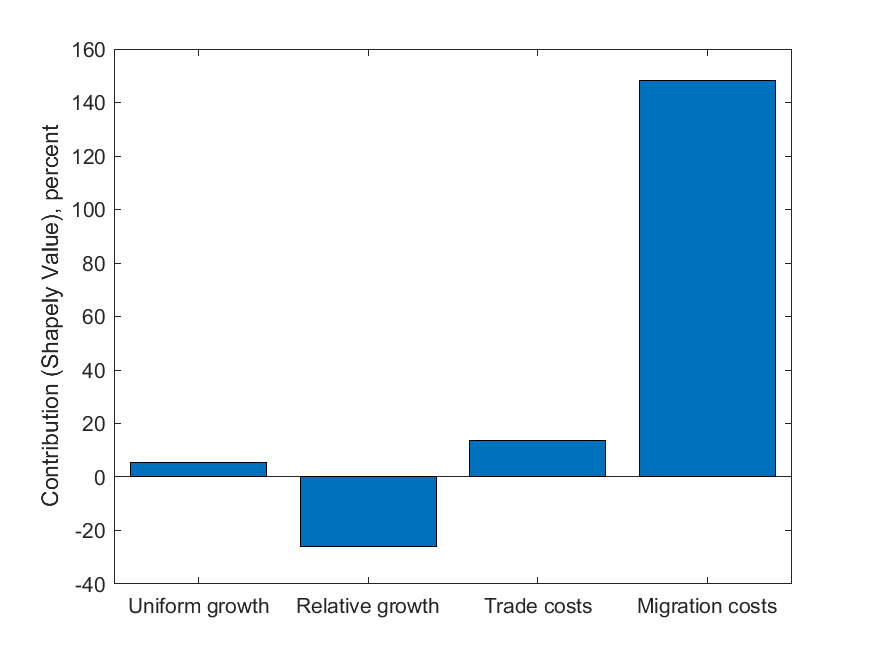
\includegraphics[width=\textwidth]{ShapelyDecomp.png}
		\caption{Shapely decomposition of the rise in density dispersion. All values add up to 100 percent. Growth in TFP and capital per worker, when uniform across provinces and set to the observed sector average, accounts for approximately 38 percent.}
		\label{fig:Shapely}
	\end{figure}



\section{Conclusion}\label{section:conclusion}
TBD




%%%BIBLIOGRAPHY%%%%%
\newpage
\clearpage
\nocite{*}
\scriptsize
\bibliography{references.bib}




\newpage
\appendix
\normalsize
\section{Proofs of Propositions}\label{appendix:proofs}

\subsection*{Proof of Proposition \ref{thm:tradeprop}}
\paragraph*{}

I start by showing that employment in both locations must be positive if there is positive employment in both sectors under Assumption \ref{assump:spatialreturns} and $1 + \theta\Omega_{n} > 0$. As mentioned before, I abstract away from equilibria where there is zero total employment in either sector. 
\begin{lem}
	Assume \ref{assump:spatialreturns} and $1 + \theta\Omega_{n} > 0$. Consider the set of equilibria where there is positive total employment in both sectors. Then employment is positive in all sector-locations and nominal output per worker equalizes across space.
\end{lem}
\begin{proof}
 Note that $1 + \theta\Omega_{a} > 0$ holds by these assumptions. Market clearing when nominal output per worker is $\phi_{i,s}$ implies, as an analogue to equation \eqref{densityclear},
\begin{equation}\label{appendix:eqclear}
	\frac{\phi_{1, s}L_{1, s}}{\phi_{2, s}L_{2, s}} = c^{\theta}\bigg[\frac{\phi_{1,s}}{\phi_{2,s}}\bigg]^{-\theta(1-\Omega_{s})}\bigg[\frac{\beta_{a}\phi_{1,a}L_{1, a} + \beta_{n}\phi_{1,n}L_{1, n}}{\beta_{a}\phi_{2,a}L_{2, a} + \beta_{n}\phi_{2,n}L_{2, n}}\bigg]^{-\theta\Omega_{s}}
\end{equation}
for every $s$. Define $Y_{i, s} = \phi_{i, s}L_{i, s}$. Fix any sequence of $\phi_{i, s} > 0$ and $Y_{i,s} > 0$ such that \eqref{appendix:eqclear} holds and $\frac{Y_{1, s}}{Y_{2, s}} \to 0$ for at least some $s$. Also assume without loss that $\sum_{i, s}Y_{i, s} = 1$. I will show that this implies that relative nominal output per worker $\frac{\phi_{1,s}}{\phi_{2,s}}$ grows without bound, making a spatial equilibrium impossible. \eqref{appendix:eqclear} can be rewritten as 
\begin{equation}\label{appendix:sequence}
	\bigg[\frac{\phi_{1,s}}{\phi_{2, s}}\bigg]^{1+\theta(1-\Omega_{s})} = c^{\theta}\bigg[\frac{\beta_{a}Y_{1, a} + \beta_{n}Y_{1, n}}{\frac{Y_{1,s}}{Y_{2, s}}(\beta_{a}Y_{2, a} + \beta_{n}Y_{2, n})}\bigg]^{-\theta\Omega_{s}}\bigg[\frac{Y_{1,s}}{Y_{2, s}}\bigg]^{-(1+\theta\Omega_{s})}
\end{equation}
The second term $\bigg[\frac{\beta_{a}Y_{1, a} + \beta_{n}Y_{1, n}}{\frac{Y_{1,s}}{Y_{2, s}}(\beta_{a}Y_{2, a} + \beta_{n}Y_{2, n})}\bigg]$ on the right hand side of this equation defines a sequence bounded within some interval $(0, b)$ for $a > 0$ and $b$ finite. Since $\Omega_{a} > 0$ this implies that relative wages in the agricultural sector diverge as relative employment $\frac{Y_{1, a}}{Y_{2, a}} \to 0$. What remains is to show that relative wages in the $n$ sector also behave in this way if $\frac{Y_{1, n}}{Y_{2, n}} \to 0$. The second term in \eqref{appendix:sequence} for the $n$ sector can be written as
\begin{equation*}
	\frac{\beta_{a}}{\beta_{a} + \beta_{n}\frac{Y_{2, n}}{Y_{2, a}}} + \frac{\beta_{n}}{\beta_{a} + \beta_{n}\frac{Y_{2, a}}{Y_{1, a}}\frac{Y_{1, n}}{Y_{2, n}}}
\end{equation*}
\paragraph*{}
Suppose for contradiction that $\frac{\phi_{1, n}}{\phi_{2,n}}$ remains bounded. A necessary condition is then that this term to tends to 0. But the only way that this is possible is if $\frac{Y_{1, a}}{Y_{2, a}} \to 0$ which we have already ruled out as supporting a spatial equilibrium. Hence, there is positive output in each sector-location. Under free mobility, this means that nominal output per worker equalizes across all sector-locations.
\end{proof}
In what follows, I search for equilibria that are interior, so that output per worker is equal across space and sectors and is normalized to 1. 

 \paragraph*{}
 I solve equations \eqref{employmentag}, \eqref{densityclear}, and \eqref{spec} to arrive at a map between relative employment in each sector as a function of total agricultural employment $\omega$. Let $\frac{L_{1, a}}{L_{2, a}} = x$. Then the equilbrium level of $x$ is implicitly defined by the relation 
 \begin{equation}
 	x = c^{\theta}\bigg[\nu(x, \omega)x + (1-\nu(x, \omega))c^{\theta\frac{\Omega_{a} - \Omega_{n}}{\Omega_{a}}}x^{\frac{\Omega_{n}}{\Omega_{a}}}\bigg]^{-\theta\Omega_{a}}
 \end{equation}
where $\nu(x, \omega)$ is the share of land in agriculture in location 2. Define the function $E(x, \omega)$ as the right hand side of the equation. Then the equilibrium value of $x$ given $\omega$ is a fixed point of $E$ given $\omega$. Moreover, it can be shown that this relation defines $x$ as a continuous function of $\omega$. It can also be shown that, when $x \in [0, c^{\theta}]$, $E(x, \omega)$ is bounded by the functions 
\begin{equation}
c^{\theta(1-\theta(\Omega_{a} - \Omega_{n}))}x^{-\theta\Omega_{n}} \leq E(x, \omega) \leq c^{\theta}x^{-\theta\Omega_{a}}
\end{equation}
 Since $\Omega_{a} > \Omega_{n}$. The set of fixed points of $E$ must then be bounded by the minimum fixed point of $c^{\theta(1-\theta(\Omega_{a} - \Omega_{n}))}x^{-\theta\Omega_{n}}$ and the maximum fixed point of $c^{\theta}x^{-\theta\Omega_{a}}$ provided these fixed points occur in the interval $[0, c^{\theta}]$. These correspond to the unique fixed points $c^{\frac{\theta(1-\theta(\Omega_{a}-\Omega_{n}))}{1 + \Omega_{n}\theta}}$ and $c^{\frac{\theta}{1 + \Omega_{a}\theta}}$, respectively, which both occur in the interval under the maintained assumption that $1 + \Omega_{n}\theta > 0$. This leads to the following lemma.
 \begin{lem}\label{append:lemspec}
 Suppose Assumption \ref{assump:spatialreturns} and $1 + \Omega_{n}\theta > 0$. Then $\frac{L_{1, n}}{L_{2, n}} > \frac{L_{1, a}}{L_{2, a}}$ in every equilibrium, and in all of such equilibria, $\frac{L_{1, a}}{L_{2, a}}$ lies in the interval $\big[c^{\frac{\theta(1-\theta(\Omega_{a}-\Omega_{n}))}{1 + \Omega_{n}\theta}}, c^{\frac{\theta}{1 + \Omega_{a}\theta}}\big]$. Lastly, $\frac{L_{1, a}}{L_{2, a}}$ attains this lower bound when $\omega = 0$. 	
 \end{lem}
 \begin{proof}
 	The second statement follows from the arguments above. The first follows from the fact that $c^{\theta\frac{(\Omega_{a} - \Omega_{n})}{\Omega_{a}}}x^{\frac{\Omega_{n}}{\Omega_{a}}} > x$ if and only if $x < c^{\theta}$. See Equation \eqref{spec}. Lastly, $\omega = 0$ implies that $\nu(x, \omega) = 0$ and thus $E(x, \omega) = c^{\theta(1-\theta(\Omega_{a} - \Omega_{n}))}x^{-\theta\Omega_{n}}$, whose fixed point in $x$ attains the lower bound.   
 \end{proof}
\paragraph*{}
We can use the lemma to bound the possible densities that can occur in equilibrium, which bound the permissible prices, to show that $\omega$ must lie on the interior of $[0, 1]$. To this end, density in sector-location $1,s$ can be written as, for $x = \frac{L_{1, a}}{L_{2, a}}$ 
\begin{equation}
d_{1, s}(\omega) = \frac{\beta_{a}\frac{x}{x + 1}\omega + \beta_{n}\frac{l(x)}{l(x) + 1}(1-\omega)}{\beta_{s}}\frac{L}{H}
\end{equation}  
where $l(x) = c^{\theta\frac{(\Omega_{a} - \Omega_{n})}{\Omega_{a}}}x^{\frac{\Omega_{n}}{\Omega_{a}}}$ as in Equation \eqref{spec}. This expression must lie in some strictly positive compact interval for every $\omega \in [0, 1]$ by the previous lemma. The same argument holds for location 2. Thus the set of permissible equilibrium log-price indices $log(P_{s})$ are bounded, as they are continuous functions of density in both locations on some strictly positive compact interval. This means that some value of $\omega$ must exist that solves Equation \eqref{agspendsh2} by the Intermediate Value Theorem. This must be the equilibrium $\omega$. 
\begin{lem}
	There exists an interior equilibrium. 
\end{lem}
\paragraph*{}
With these caveats out of the way, I can finally show that growth in the TFP terms $a_{i, s}$ tend the equilibrium level of $\omega \to 0$. To this end, the equilibrium level of $\omega$ can be written as the solution to Equation \eqref{agspendsh2}
\begin{multline}\label{appendix:equilibrium}
log(\omega) - \epsilon_{a}\log(1 -\omega) = -(1-\eta)\log(a_{a}) + (1-\eta)\epsilon_{a}log(a_{n}) + \\ -(1-\eta)\frac{1}{\theta}\log\bigg[c^{\theta}d_{1, a}(\omega)^{-\theta\Omega_{a}} + d_{2, a}(\omega)^{-\theta \Omega_{a}}\bigg] + (1-
\eta)\epsilon_{a}\frac{1}{\theta}\log\bigg[c^{\theta}d_{1, n}(\omega)^{-\theta\Omega_{n}} + d_{2, n}(\omega)^{-\theta \Omega_{n}}\bigg]
\end{multline}
where the density terms on the second line are bounded over all $\omega$. By Assumption \ref{assump:growthrates}, the terms $-(1-\eta)\log(a_{a}) + (1-\eta)\epsilon_{a}\log(a_{n})$ decrease without bound with respect to time. This immediatley implies that all possible $\omega$ solving \eqref{appendix:equilibrium} must lie in some interval $(a, b)$ where $a \to 0$ and $b \to 0$. 
\begin{lem}
	Suppose Assumption \ref{assump:growthrates} holds. Then the set of possible equilibrium $\omega$ lie in the interval $(a, b)$ where $a \to 0$ and $b \to 0$.  
\end{lem}
I can now prove the entire proposition. Total employment in location 1 can be written in terms of $x$ and $\omega$,
\begin{equation}
	L_{1, a} + L_{1, n} = \bigg[\frac{x}{x + 1}\omega + \frac{l(x)}{l(x) + 1}(1-\omega)\bigg]L
\end{equation}
I will show that this term approaches a maximized value when $\omega \to 0$. Lemma \eqref{append:lemspec} implies that $x$ attains its minimum value when $\omega = 0$ and also implies $l(x) > x$. Assumption \ref{assump:spatialreturns} implies that $l(x)$ is strictly decreasing in $x$, and thus reaches its maximum value when $\omega = 0$. Let $x_{min}$ a be the minimum possible value of $x$ given by the interval in Lemma \eqref{append:lemspec}. Then the following set of inequalities holds
\begin{equation}
	\frac{x}{x + 1} < \frac{l(x)}{l(x) + 1} < \frac{l(x_{min})}{l(x_{min}) + 1}
\end{equation}    
for every $\omega \in (0, 1)$ and so
\begin{equation}
\bigg[\frac{x}{x + 1}\omega + \frac{l(x)}{l(x) + 1}(1-\omega)\bigg]L < \frac{l(x_{min})}{l(x_{min}) + 1}L
\end{equation}
for every $\omega \in (0, 1)$. Since the implicit function $x(\omega)$ is continuous in $\omega$, 	$L_{1, a} + L_{1, n}$ approaches this maximum value $\frac{l(x_{min})}{l(x_{min}) + 1}L$ as $\omega \to 0$. This completes the proof. 
\paragraph*{}

\newpage

\section{Additional Figures and Tables} \label{appendix:figures}

	\begin{figure}[h]
		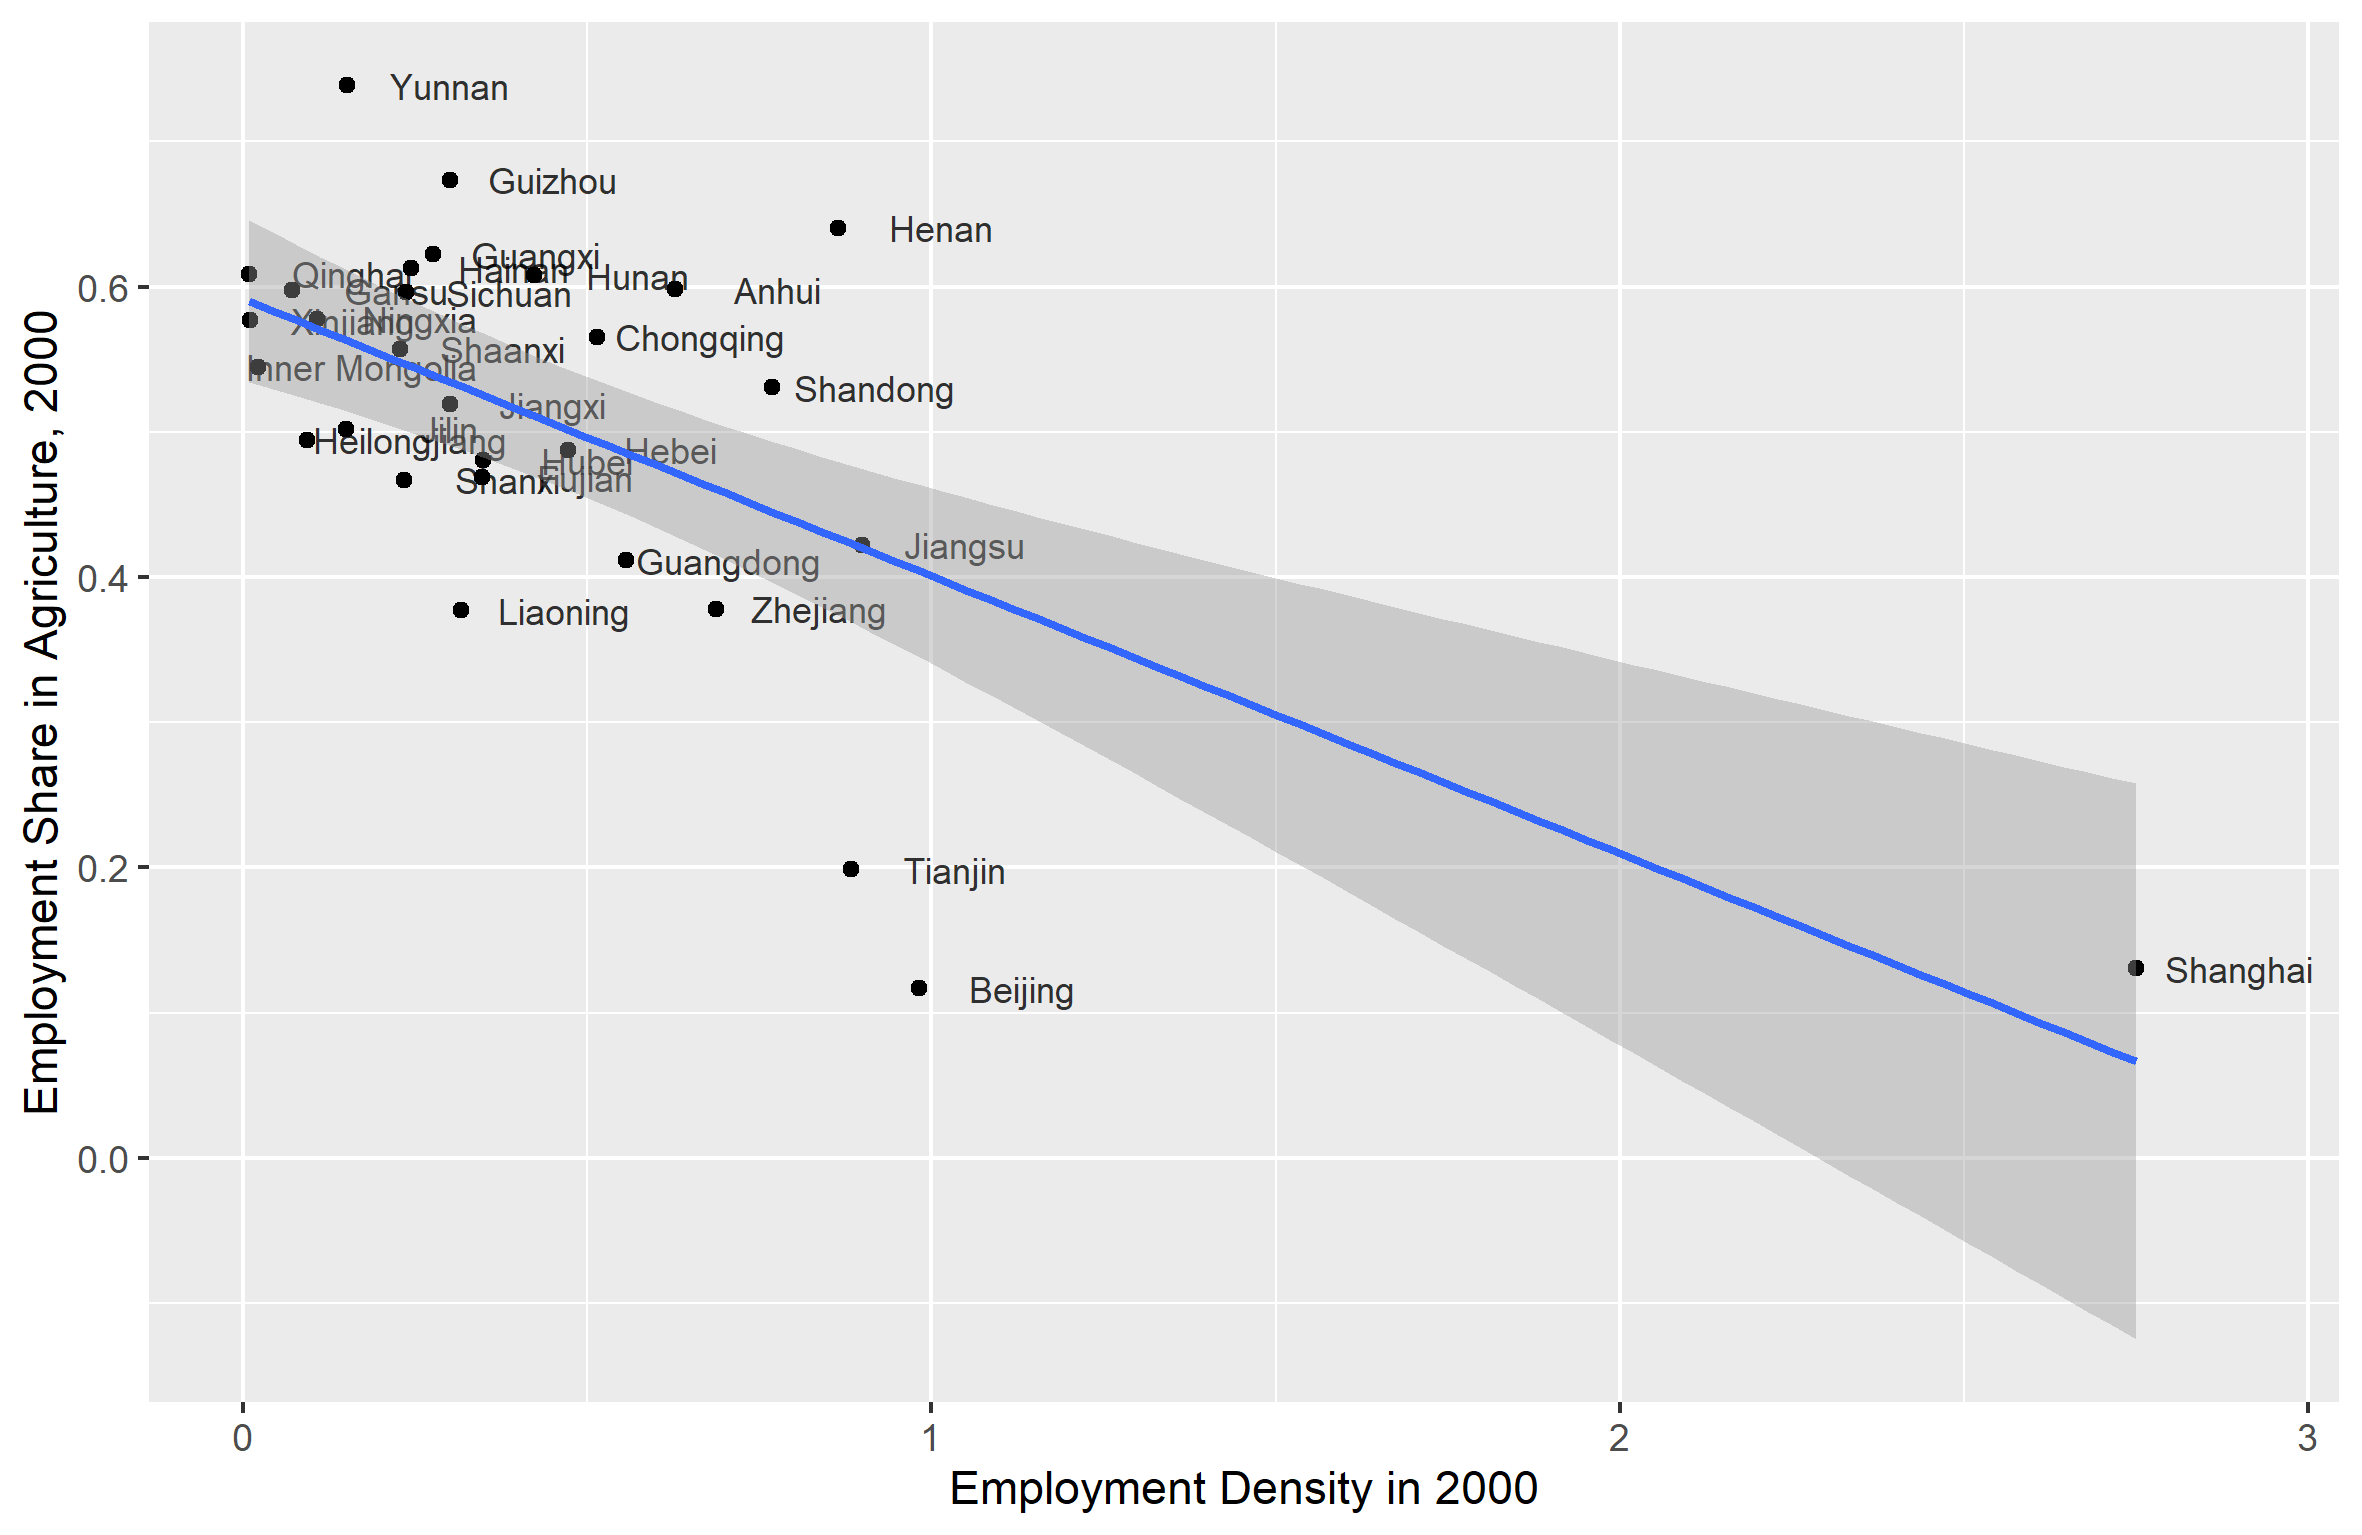
\includegraphics[width=\textwidth]{fig1.png}
		\caption{Relationship between primary sector employment and initial employment density by Chinese province. Density is measured in millions per 1000 square miles. The model explains greater than 45 percent of the variation in agriculture employment shares. Similar results hold for the 2005 cross section.}
		\label{fig:emp_share_dens}
	\end{figure}
\newpage
\begin{figure}[h]
	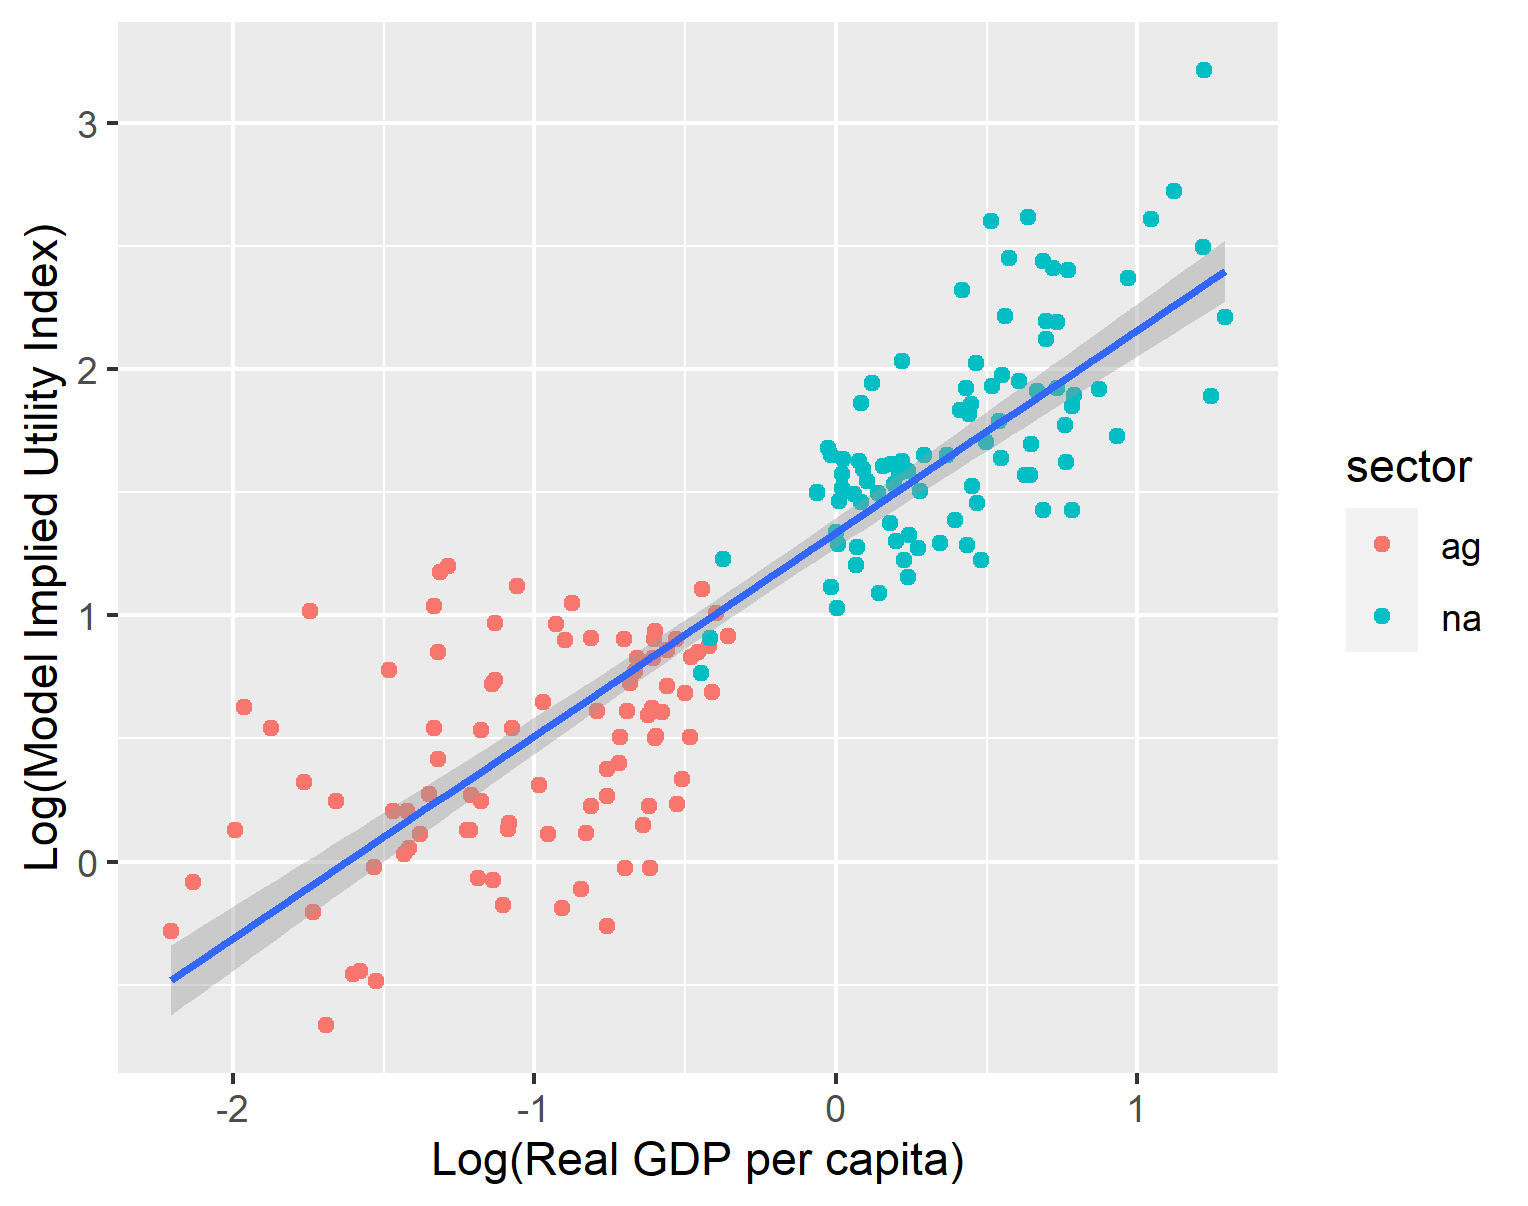
\includegraphics[width=\textwidth]{model_implied_index.png}
	\caption{Relationship between model implied real GDP of goods consumption against real income per capita constructed in \cite{tombezhu}. Sector "ag" corresponds to agricultural workers. The model implied index is constructed using the relation $\log(U_{ist}) = \log(\phi_{is, t}) - \log(P_{in, t}) + \frac{1}{1-\hat{\eta}}\log[1-\omega_{is,t}]$ implied by Equation \eqref{agspendsh2}. $R^{2}$ of the regression is over 55 percent. }   
	\label{fig:model_implied_index}
\end{figure}

\begin{figure}

		\makebox[\textwidth][c]{\begin{tabular}{||c c c c c||}
			\hline
			$\epsilon_{a}$ & $\eta$ & $\lambda_{2000}$ & $\lambda_{2005}$ & $\lambda_{2010}$ \\
			\hline \hline
			1.875 & 1.698 & 0.875 & -0.157 & 0.017 \\
			
			[0.832, 3.459] & [1.437, 2.073] &[-0.2665, 2.2918]  & [-0.4774, 0.227] & [-0.5304, 0.6492] \\
			\hline
		\end{tabular}}

	\caption{Estimates under the specification used in \cite{cominetal2021}. Assuming perfect mobility within locations but not across them, as well as no trade, their estimating equation is instead $log\bigg[\frac{L_{iat}}{L_{int}}\bigg] =  (1-\eta)log\bigg[\frac{P_{iat}}{P_{int}}\bigg] +  (1-\eta)(\epsilon_{a} - 1)log\bigg[\frac{\phi_{ist}}{P_{int}}\bigg] + (\epsilon - 1)log(1-\omega_{ist}) + \sum_{t}\lambda_{t} + log(v_{ist})$. I do not introduce sector trade controls that they do, and these do not affect their estimates. 99 percent BCa confidence intervals are reported. This equation is estimated using only the non-agricultural subsample because there is no within-province variation in the dependent variable. These results imply that the entire fall in spending shares can be explained by substitution effects.}
	\label{fig:cominestimate}
\end{figure}


\begin{figure}
	\makebox[\textwidth][c]{\begin{tabular}{||c c c c c||}
		\hline
		&$\Delta$M = 0, $\Delta$R= 0 & $\Delta$M = 0, $\Delta$R = 1 & $\Delta$M = 1, $\Delta$R = 0 & $\Delta$M = 1, $\Delta$R = 1 \\
		\hline
		$\Delta$T = 0, $\Delta$A = 0 &1.0646 &0.9998 &1.2039 &1.0990  \\
		$\Delta$T = 0, $\Delta$A = 1 &1.0953 &1.0033 &1.2597 &1.1046  \\
		$\Delta$T = 1, $\Delta$A = 0 &1.0826 &1.0121 &1.2327 &1.1196  \\
		$\Delta$T = 1, $\Delta$A = 1 &1.1126 &1.0160 &1.2860 &1.1259 \\
		\hline
	\end{tabular}}
	\caption{Table of equilibrium population density dispersion, measured in the coefficient of variation of population density across provinces. $\Delta A$ corresponds to uniform growth, $\Delta R$ corresponds to relative growth, $\Delta M$ to changes in migration costs and $\Delta T$ to changes in trade costs.}
	\label{fig:marginaleffects}
\end{figure}

\clearpage
\newpage
\section{Equilibrium Description and Computation}\label{appendix:eqdefcomp}
\paragraph*{}
\subsection*{Definition}
\paragraph*{}

In this appendix, I detail the system of equations in 2005 that is used to construct the counterfactual equilibria. All variables are defined in Section \ref{section:structmodel}, which I repeat here for convenience. As is standard notation, variables with hats denote values in 2005 relative to values in 2000. The endogenous variables determined in equilibrium are output per worker $\hat{\phi_{is}}$, change in employment $\hat{L_{is}}$, marginal costs $\hat{c_{is}}$, price indices $\hat{P_{i,s}}$, housing production and consumption allocations $\hat{H_{is}}$ and $\hat{H^{c}_{is}}$, and rental rates $\hat{r_{i}}$, and 2005 spending shares on sector $k$ goods $\omega^{k}_{is}$ and migration flows $m_{isjk}$. I start with the marginal cost pricing condition, for location $i$ and sector $s$,

\begin{equation}
	\hat{p_{is}} = \hat{c_{is}} = \frac{\hat{\phi_{is}}^{v_{s}}\bigg[\frac{\hat{L_{is}}}{\hat{H_{is}}}\bigg]^{\beta^{H}_{s}}\bigg[\frac{\hat{L_{is}}}{\hat{K_{is}}}\bigg]^{\beta^{K}_{s}}\hat{P_{ia}}^{\beta_{as}}\hat{P_{in}}^{\beta_{ns}}}{\hat{a_{is}}\bigg[\frac{\hat{L_{is}}}{\hat{H_{is}}}\bigg]^{\alpha_{s}}}	
\end{equation}
where $v_{s}$ is the value added share in sector $s$. We have the price index equation, which can be written in hat-algebra form
\begin{equation}
	\hat{P_{is}} = \bigg[\sum_{j \in \mathbf{P}}\pi_{ji,s2000}\hat{\tau_{ji,s}}^{-\theta_{s}}\hat{c_{js}}^{-\theta_{s}}\bigg]^{-\frac{1}{\theta_{s}}}
\end{equation}
and a system of equations that implies the goods market clearing and balanced trade, represented in hat-algebra form for all $i$ and $s$,

\begin{equation}
\begin{aligned}
	\hat{\phi_{is}}\hat{L_{is}}\frac{\phi_{is, 2000}L_{is, 2000}}{v_{s}} =  \\ 
	\sum_{j \in \mathbf{P}, k \in \{a, n\}}\bigg[\omega^{s}_{jk} + \beta_{s k}\frac{1}{v_{k}}\bigg]\bigg[\hat{\phi_{jk}}\hat{L_{jk}}\phi_{jk, 2000}L_{jk, 2000}\bigg] \frac{\pi_{ij, s, 2000}\hat{\tau_{ij, s}}^{-\theta_{s}}\hat{c_{i, s}}^{-\theta_{s}}}{\sum_{l \in \mathbf{P}}\pi_{lj, s, 2000}(\hat{\tau_{lj,s}})^{-\theta_{s}}\hat{c_{l, s}}^{-\theta_{s}}}
\end{aligned}
\end{equation}
where $\phi_{is, 2000}$ is the output per worker uniquely constructed to balance trade in 2000 given trade flow data, with $L_{is, 2000}$ and $\pi_{is, 2000}$ being employment and trade flow data in 2000, and $\omega^{k}_{is, 2000}$ the observed spending share in sector $k$ in 2000.
\paragraph*{}
Agriculture spending shares in China are determined by the equation (noting that the preference parameter $\gamma_{is}$ is time invariant) 
\begin{equation}
	\begin{aligned}
	\log\omega^{a}_{is} - \epsilon_{a}\log(1-\omega^{a}_{is}) = \\ (1-\eta)\log\bigg[\frac{\hat{P_{ia}}}{\hat{P_{in}}}\bigg] + (\epsilon_{a}-1)(1-\eta)\log\bigg[\frac{\hat{\phi_{is}}}{\hat{P_{in}}}\bigg] + \log\omega^{a}_{is,2000} - \epsilon_{a}\log(1-\omega^{a}_{is,2000})
	\end{aligned}
\end{equation}
where the international spending share remains exogenous at world value added. Migration flows, as a fraction of total hukou registrants in $(j,k)$ in 2005, can be described as follows (in hat algebra form), 
\begin{equation}
m_{jkis} = \frac{(\hat{W_{is}}/\hat{f_{jkis}})^{\kappa}}{\sum_{i' \in \mathbf{P} \backslash \{RoW\}, s'\in \{a, n\}}(\hat{W_{i's'}}/\hat{f_{i's'is}})^{\kappa}m_{i's'is, 2000}}
\end{equation}
where $m_{isjk,2000}$ are migration flows in the data. The welfare index $\hat{W_{is}}$ satisfies
\begin{equation}\label{welfareindex}
	\hat{W_{is}} = \frac{\hat{\phi}_{is}}{\bigg[\sum_{k \in \{a, n\}}\omega_{is, 2000}^{k}\hat{P}_{ik}^{1-\eta}\bigg]^{\frac{\nu}{1-\eta}}\hat{r_{i}}^{1-\nu}}
\end{equation}
labour market clearing in 2005 implies
\begin{equation}
	\hat{L_{is}}L_{is, 2000} = \sum_{i' \in \mathbf{P} \backslash \{RoW\}, s'\in \{a, n\}}m_{i's'is}M_{i's', 2005}
\end{equation}
where $M_{is, 2005}$ is the inferred stock of individuals with the corresponding hukou in 2005, which is exogenous. Finally, $\hat{r_{i}}$ is determined by the unique land allocation  $\hat{H_{is}}$ and $\hat{H^{c}_{is}}$ that equates marginal products with the price of land in consumption. 
\paragraph*{}
An equilibrium allocation is defined as a solution to each equation in the endogenous variables as a function of $\hat{K_{is}}$, $\hat{a_{is}}$, $\hat{f_{is,jk}}$ and $\hat{\tau_{ij, s}}$.


\subsection*{Computation}

\subsection*{Derivation of Welfare Index}
\paragraph*{}
I define $CV_{is}$ as the fraction of income deducted in 2005 in order for a worker in $(i,s)$ to be as well off as in 2000. Let $E_{is}(P, V)$ denote the minimum expenditure required to achieve consumption level $V$ at prices $P$ for workers in $(i, s)$. This is derived from the utility function in Equation \eqref{preferenceshouse} with preference parameters $\gamma_{is}$ allowed to vary. Then, $\tilde{CV_{is}}$ is defined by the equation
\begin{equation}\label{cv}
	(1-CV_{is})\frac{\phi_{is, 2005}}{1-\nu} = E(P_{is, 2005}, V_{2000})
\end{equation}
where $V_{2000}$ is the utility achieved in 2000 under time-invariant preferences, $\phi_{is, 2005}$ value added per worker in 2005 (in this case proportional to nominal income because land spending is rebated and preferences over housing are Cobb-Douglas) and $P_{is, 2005}$ are the prices faced by workers in 2005. Define $\mathbf{P}_{is}(P, V) = \frac{E_{is}(P, V)}{V}$ as the \textit{price index} associated with the level of utility $V$ and prices $P$. Also note by duality, $\phi_{is, 2005} = E(P_{is, 2005}, V_{2005})$. Then \eqref{cv} can be re-written as
\begin{equation}\label{cvrewrote}
		\frac{1}{1-CV_{is}} = \frac{\hat{\phi_{i, s}}}{\hat{\mathbf{P_{is}}}(V_{2000})}
\end{equation}
Where $\hat{\mathbf{P_{is}}}(V_{2000})$ is the proportional change in the price index \textit{holding utility constant at 2000 levels}. If preferences are homothetic, this change in price index is constant in $V$ and so \eqref{cvrewrote} reduces to the proportional change in utility $\hat{V}$ \citep{samswamy}. However, since preferences are not homothetic, the price index will depend on the initial level of utility $V_{2000}$ which breaks the connection with $\hat{V}$. 
\paragraph*{}
I now derive the price index $\hat{\mathbf{P_{is}}}$. To do this, I need to define a second price index associated only with goods consumption, with the measure of goods consumption coming from the non-homothethic CES in Equation \eqref{preferences}. Call this index $\mathbb{P}_{is}(P, U)$ associated with prices $P$ and goods consumption level $U$. The connection with $\mathbf{P_{is}}$ and $\mathbb{P}_{is}$ is derived, noting that preferences over goods and housing is Cobb Douglas,
\begin{equation}
	\mathbf{P_{is}} = \mathbb{P}_{is}(P, U)^{\nu}r_{i}^{1-\nu}
\end{equation} 
and so
\begin{equation}\label{goodsaggregatelink}
	\hat{\mathbf{P_{is}}}(V_{2000}) = \hat{\mathbb{P}_{is}}( U_{2000})^{\nu}\hat{r_{i}}^{1-\nu}
\end{equation} 
It remains to solve for $\hat{\mathbb{P}_{is}}( U_{2000})$, which is the change in the goods price index holding the measure of goods consumption $U$ at 2000 levels. This can be written directly as (via the solution to the consumers problem)
\begin{equation}\label{welfareindexsolution}
\hat{\mathbb{P}_{is}}(U_{2000}) =	\frac{\bigg[\sum_{k \in \{a, n\}}U_{2000}^{(\epsilon_{k} - 1)(1-\eta)}P_{ik, 2005}^{1-\eta}\bigg]^{\frac{1}{1-\eta}}}{\bigg[\sum_{k \in \{a, n\}}U_{2000}^{(\epsilon_{k} - 1)(1-\eta)}P_{ik, 2000}^{1-\eta}\bigg]^{\frac{1}{1-\eta}}}
\end{equation}
However, solving the consumers problem also implies $\omega^{k}_{is, 2000} = \frac{U_{2000}^{\epsilon_{k} (1-\eta)}P_{ik, 2000}^{1-\eta}}{\bigg[\frac{\phi_{is, 2005}}{1-\nu}\bigg]^{1-\eta}}$, which coupled with the definition $\bigg[\sum_{k \in \{a, n\}}U_{2000}^{(\epsilon_{k} - 1)(1-\eta)}P_{ik, 2000}^{1-\eta}\bigg]^{\frac{1}{1-\eta}} = \frac{\phi_{is, 2000}}{U_{2000}(1-\nu)}$  and subbing both into Equation \eqref{welfareindexsolution} yields the index measure 
\begin{equation}\label{goodsindex}
\hat{\mathbb{P}_{is}}(U_{2000}) = \bigg[\sum_{k \in \{a, n\}}\omega_{is, 2000}^{k}\hat{P}_{ik}^{1-\eta}\bigg]^{\frac{1}{1-\eta}}
\end{equation}
Substituting \eqref{goodsindex} into \eqref{goodsaggregatelink} and then into \eqref{cvrewrote} yeilds the welfare index formula used in \eqref{welfareindex}.
\end{document}
